\section{NUMERICAL EXPERIMENTS}

\subsection{Experiment \# 0: Linear Diffusion}

In this section the enunciated homogenization theorem will be numerically validated first in a linear setting (only diffusion). To do this, we can write the problem \eqref{eq:MDE} neglecting the reaction term and using the following variational approach: find  $\phi^{n+1}$ such that:

\begin{equation}
\int_{\Omega} \phi^{n+1} ~v ~d \Omega+ \Delta t \int_{\Omega} (D \nabla \phi^{n+1}) \cdot \nabla v ~ d \Omega  = \int_{\Omega} \phi^{n} v ~ d \Omega + \Delta t  \int_{\Gamma_N} g v ~ ds  \label{eq:diff_weak_form}
\end{equation}

where $v \in V$, $V = \{ v \in H^1(\Omega)\}$. The Backward Euler method was used to discretize the temporal variable, i.e., $\dot{\phi} = (\phi^{n+1} - \phi^{n})/\Delta t$, where $\Delta t$ is the time step and $\phi^{n+1}$ is the resolved potential field at the previous time-step.

Let us start by setting a two-dimensional problem ($d = 2$) considering $\Omega = [0,25 \text{mm}]\times[0, 25 \text{mm}]$. The diffusion tensor will be taken as \eqref{eq:macroscopic_diff_tensor}, using the parameters of table \ref{tab:parameters_tensor}:

\begin{table}[!htbp]
	\centering
	\caption{common parameters for numerical experiments.}
	\label{tab:parameters_tensor}
	\begin{tabular}{@{}ccc@{}}
		\toprule
		Paramter & Meaning                & Value        \\ \midrule
		$d_1$    & main fiber diffusivity & 0.1  $[mm/s]$ \\
		$\gamma$ & defined below   & 4            \\
		$\beta$ & defined below           & 5            \\
		$\hat{f}$ & main fiber direction  & $(1,~0)$           \\
		$\hat{c}$ & cross fiber direction & $(0,~1)$            \\ 
		$I_{dur}$ & stimulus duration    & 3 $[ms]$           \\
		$a$ & radius of the myocites array with collagen & 0.1  [mm]       \\ 
		$b$ &\begin{tabular}[c]{@{}c@{}}distance between the start of two contiguous collagen\\ inclusions (in direction $e_2$)\end{tabular}    & 1 [mm]  
		\\ \bottomrule
	\end{tabular}
\end{table}


where $\beta$ is defined by $d_{col} = 10^{-\beta} \times d_1$ and $d_2 = d_1/\gamma$. So, the collagen diffusion tensor is taken as $D_{col} = d_{col} \times \mathbb{I}_2$. The boundary condition is taken as a constant Neumann stimulus at the left edge of intensity $I_{est} = 50$ and duration $I_{dur}$. In the other boundaries just zero Neumann boundary conditions are asumed. Also, zero initial conditions are assumed over all the domain.

The geometry for simulation is shown in figure \ref{fig:geometry}. The materials proportions were chosen as $\theta_c = 0.4$ and $\theta_f = 0.5$ (highly fibrotic tissue). The time step is $1~[ms]$.

\begin{figure}[!htbp]
	\centering
	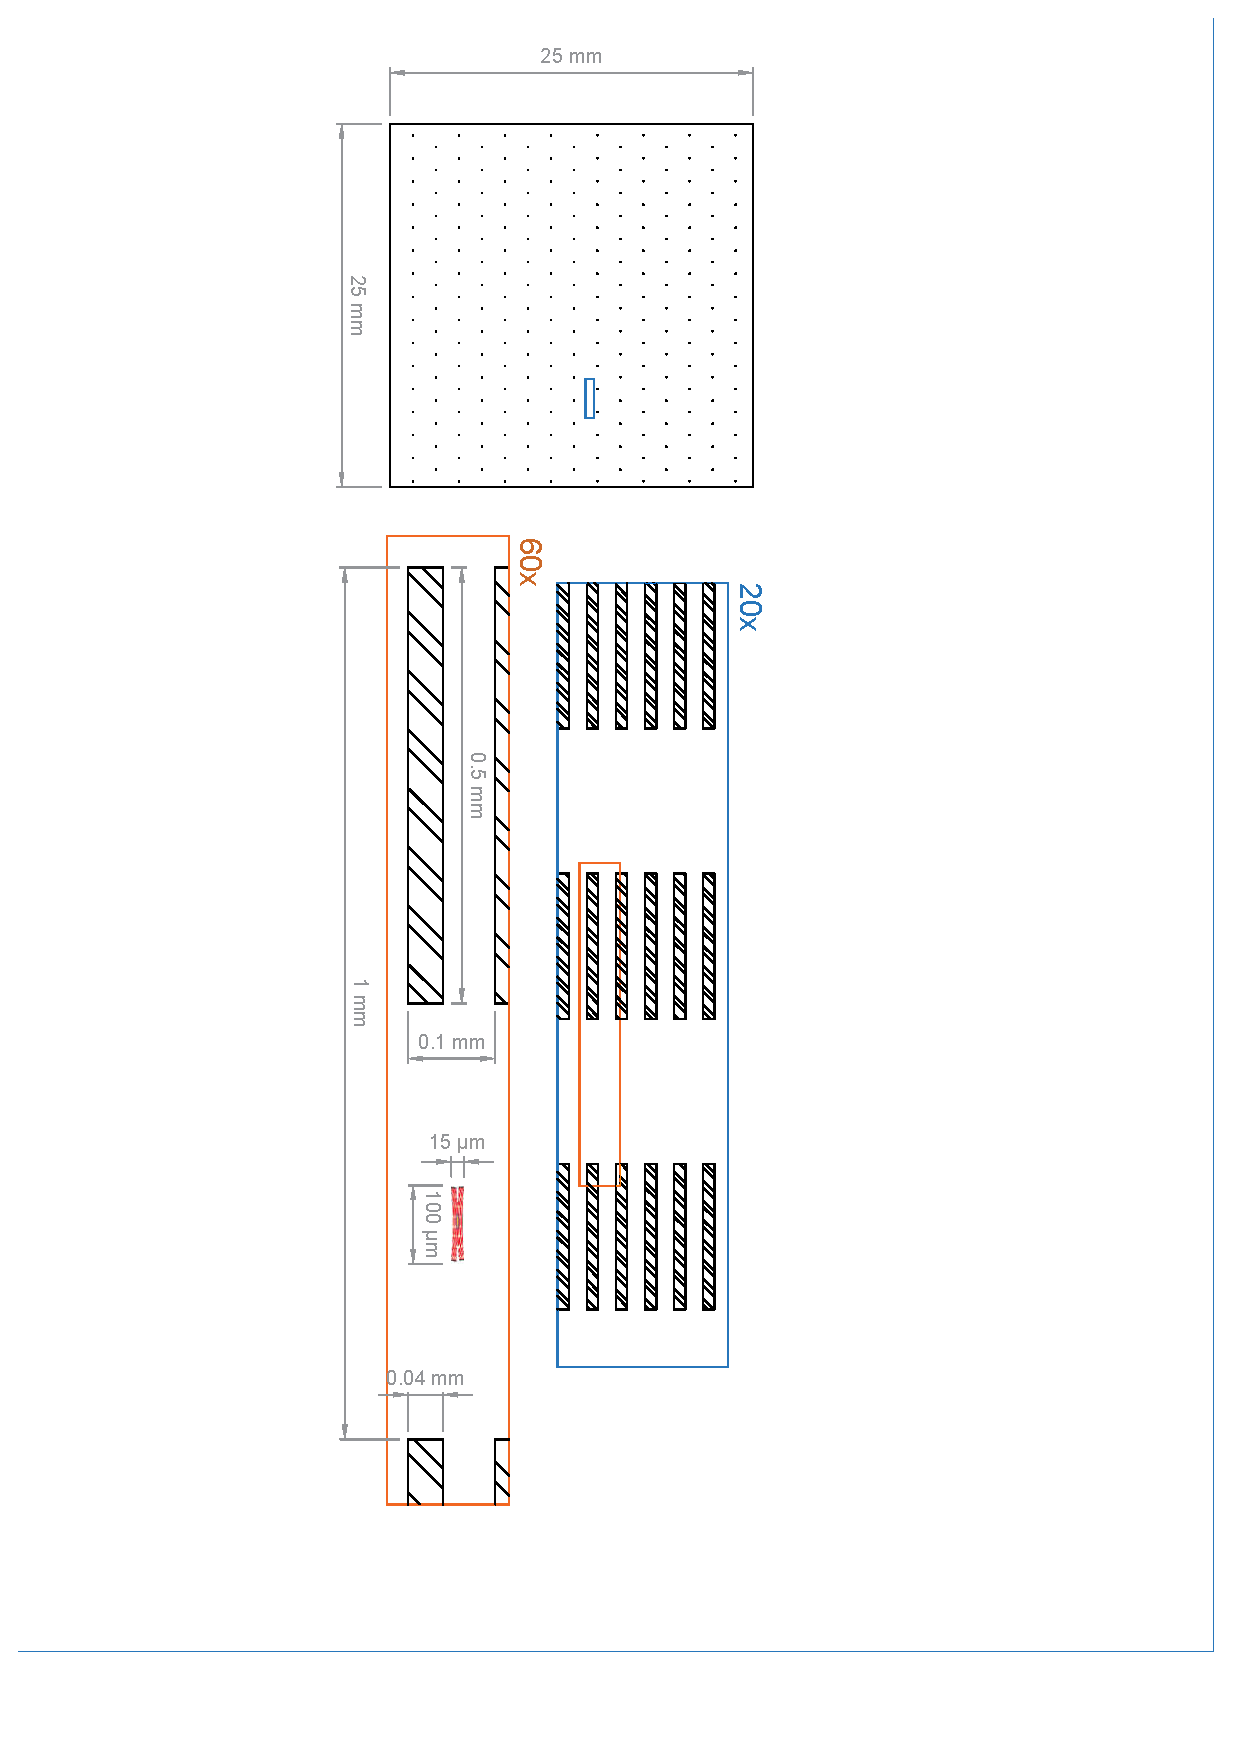
\includegraphics[trim={5cm 2cm 7cm 0.5cm}, clip, width = 5.4 cm, angle = 90]{fig/Verificacion_Teorema/geometry}
	\caption{geometry used to solve the exact problem. } \label{fig:geometry}
\end{figure}

A unstructured mesh composed by triangles of 0.1 [mm] characteristic size is used for the exact problem, which is refined near collagen inclusions in order to correctly consider the meso-scale into the model. Refined elements has a characteristic size of 0.0075 [mm]. On the other hand, the mesh used to solve the homogenized problem has a characteristic length of 0.1 [mm]. This difference is a consequence of the fact that homogenized model does not need explicitly the mesoscale in the mesh, because the mesoscopic properties are already considered in the effective macroscopic diffusion tensor. The mesh size for the homogenized problem is selected in order to have at least (usually more) one node per each inclusion, which is useful for randomly generated fibrotic meshes, that will be used in some experiments. For this case, a even more coarse mesh can be used, given the constant value of $\theta_c$ and $\theta_f$.

In order to quantify the approximation error at each time step, we can use the L2-norm, this is:

\begin{equation}
\text{error} = \frac{\norm{\phi - \phi_h}_{L2}}{\norm{\phi}_{L2}} = \frac{\int_{\Omega} (\phi - \phi_h)^2 d\Omega}{\int_{\Omega} \phi^2 d \Omega} \label{eq:errorL2}
\end{equation}

The final error obtained has three sources: the homogenization, the use of a coarse mesh in the homogenized problem, and the interpolation of the exact solution in the coarser mesh in order to calculate the error. Is mandatory to isolate the homogenization error from the mesh produced error. We did this by solving the equations over a tissue without collagen ($\theta = 0$). So, with this result, we chooses the mesh described above keeping the L2$-$error of the mesh coarseness below $10^{-2}$.

\begin{figure}[!htbp]
	\centering
	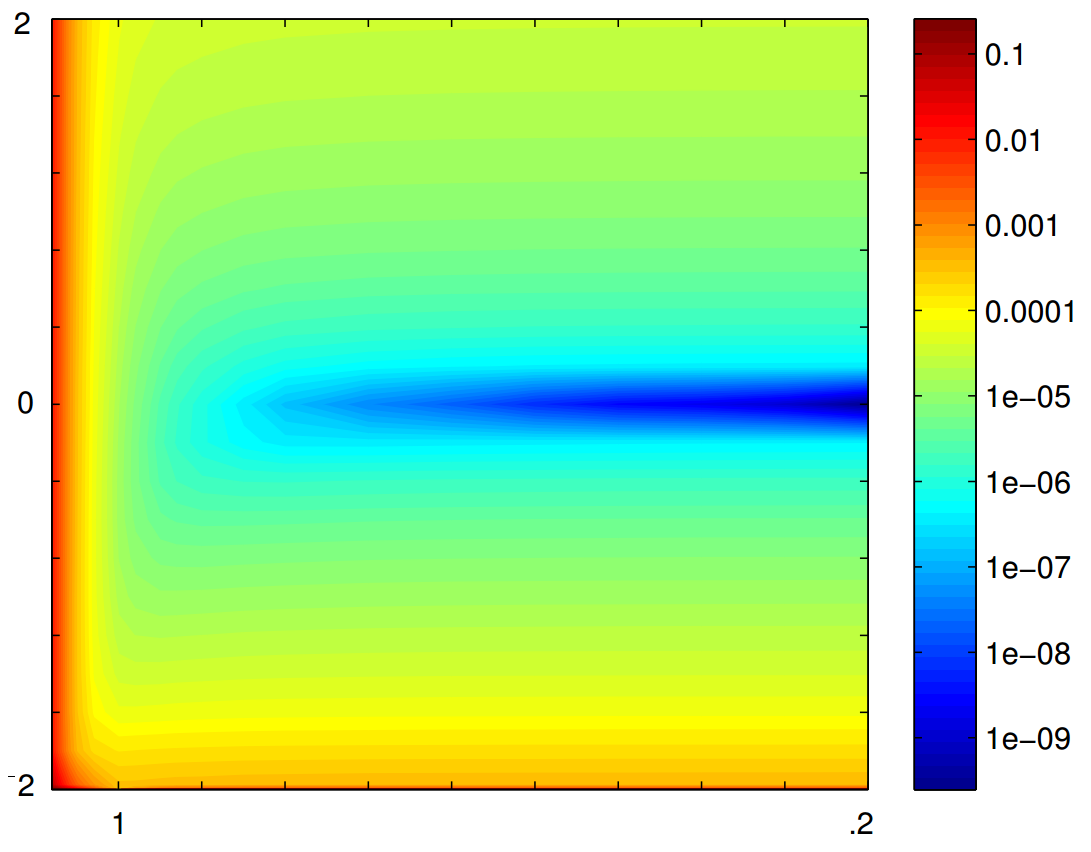
\includegraphics[height = 4.5 cm]{fig/Verificacion_Teorema/comparison_MEJORAR_SI_ALCANZO}
	\caption{Plot of L2-error for different mesh sizes and $\beta$ values (log scale on $\phi$). The horizontal axis has the mesh refinement in millimeters. The vertical axis has the $\beta$ values.} \label{fig:errorR1}
\end{figure}


In order to verify the established above, we  can solve the stationary version of \eqref{eq:diff_weak_form} for different mesh sizes and $\beta$ values, as can be seen in th Figure \ref{fig:errorR1}, where we can see that the homogenized solution converges to the exact one when $\beta \rightarrow 0$ and mesh size becomes equal to the mesh size for the exact problem.

\begin{figure}[!htb]
	\centering
	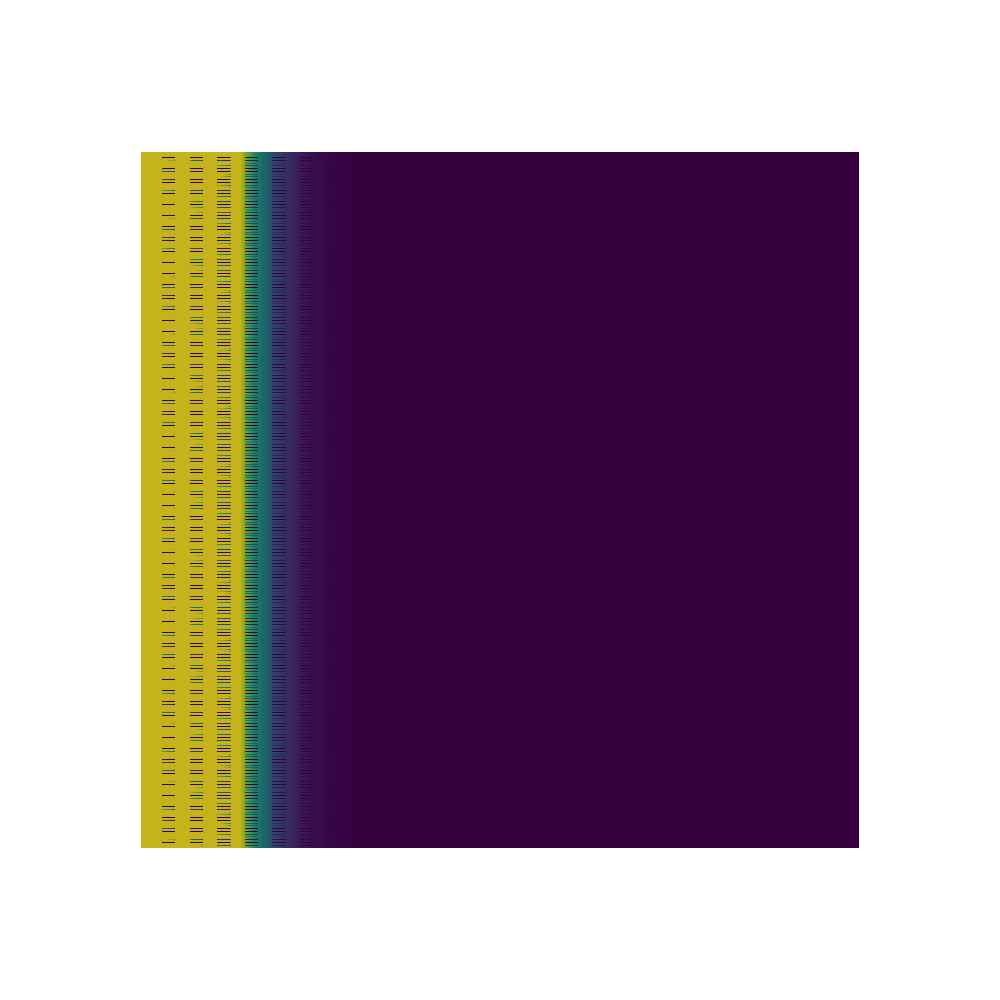
\includegraphics[height = 3 cm, trim = {6cm 6cm 6cm 6cm}, clip]{fig/Verificacion_Teorema/20}
	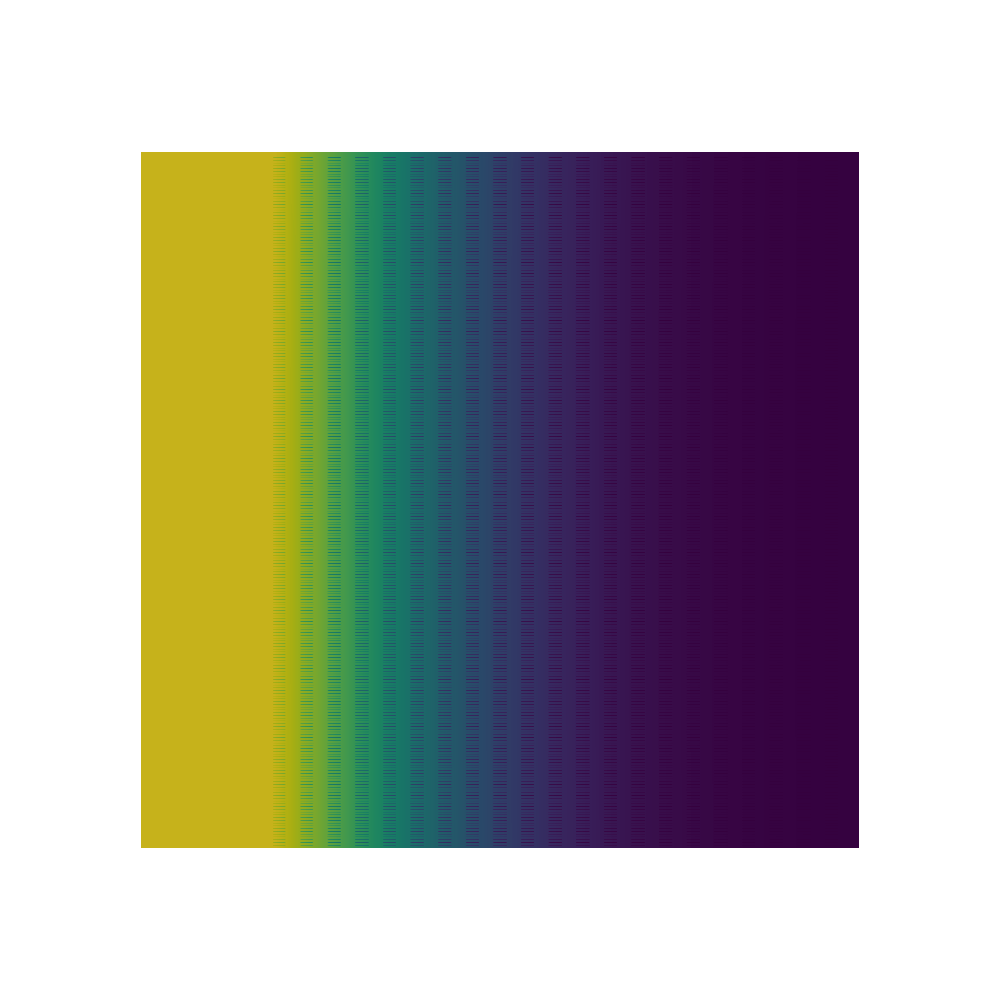
\includegraphics[height = 3 cm, trim = {6cm 6cm 6cm 6cm}, clip]{fig/Verificacion_Teorema/250}
	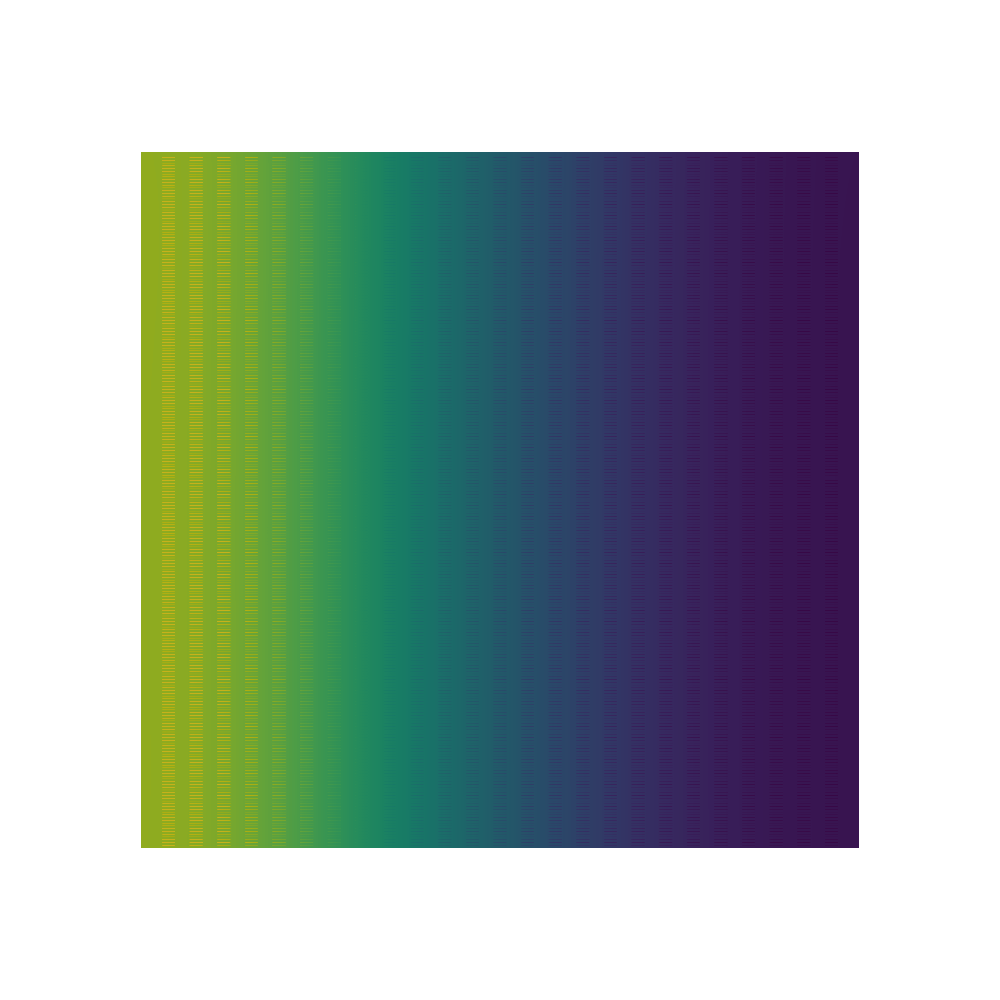
\includegraphics[height = 3 cm, trim = {6cm 6cm 6cm 6cm}, clip]{fig/Verificacion_Teorema/500}
	
\includegraphics[height = 3 cm, trim = {6cm 6cm 6cm 6cm}, clip]{fig/Verificacion_Teorema/700}
	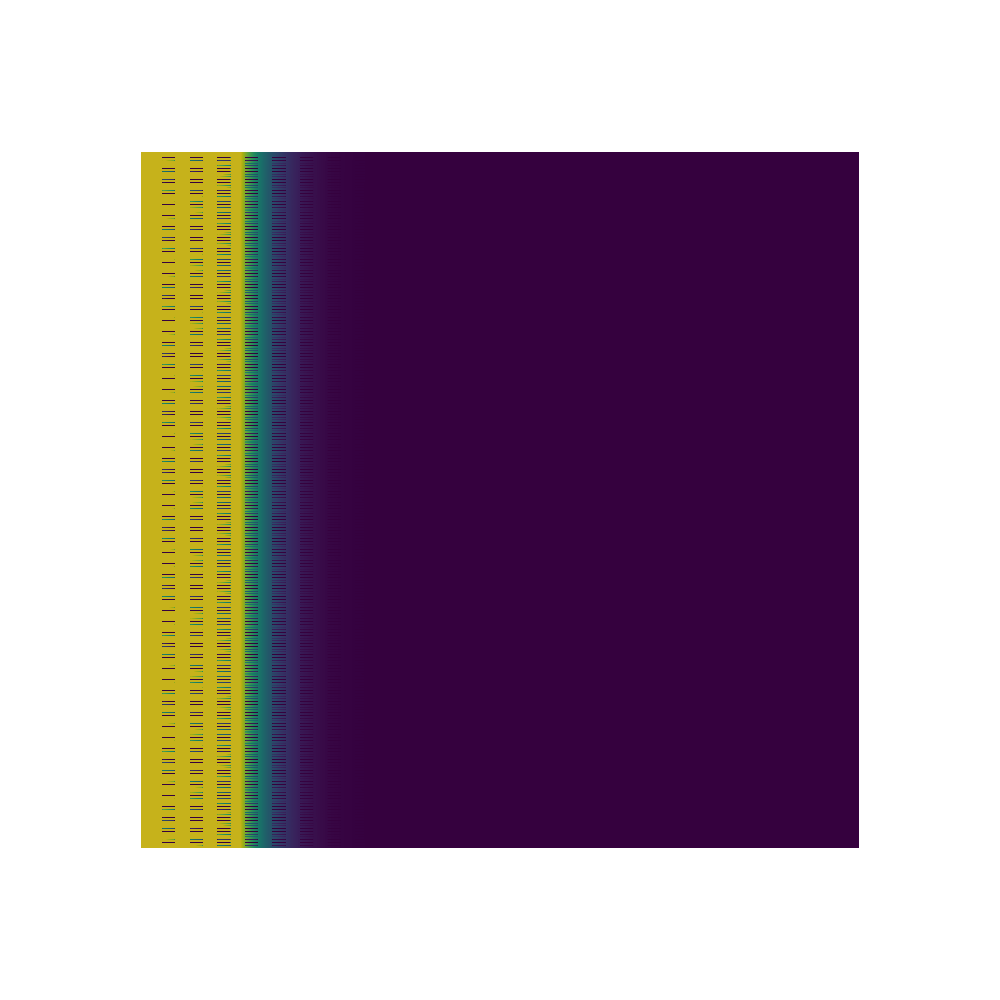
\includegraphics[height = 3 cm, trim = {6cm 6cm 6cm 6cm}, clip]{fig/Verificacion_Teorema/20h}
	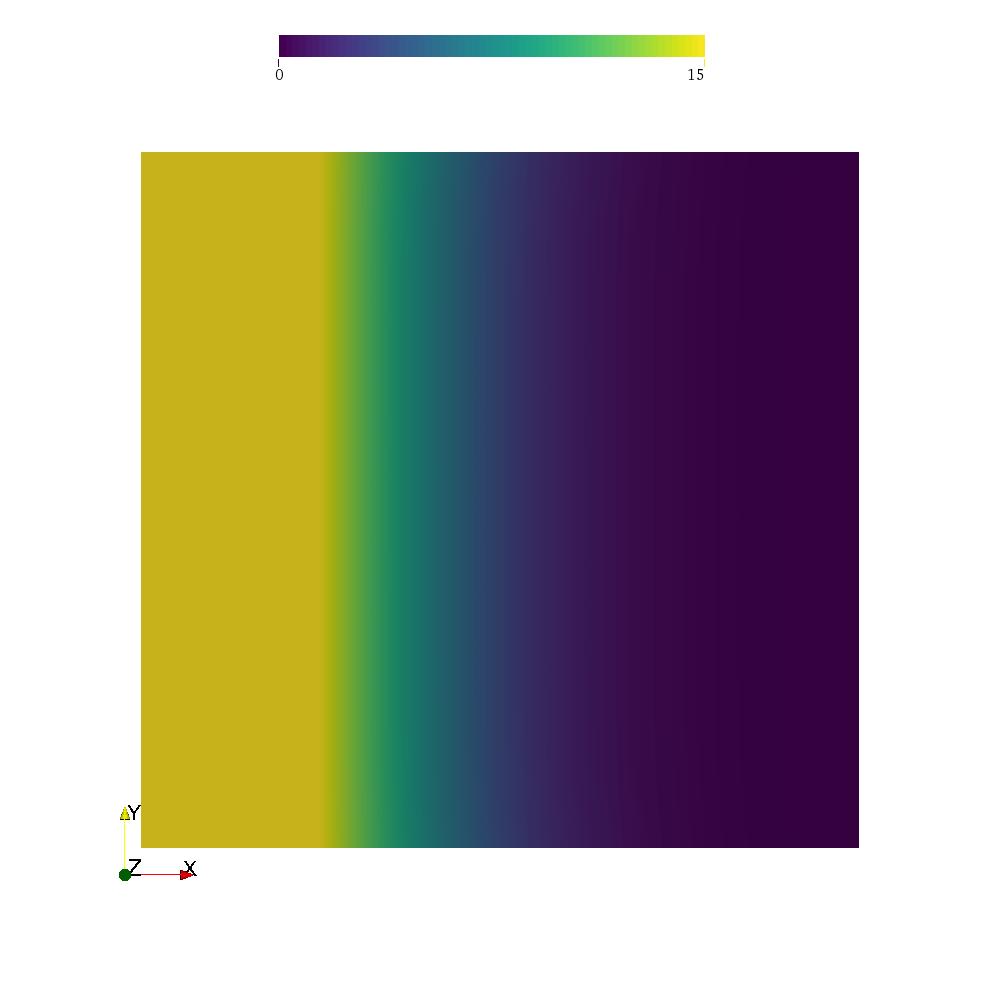
\includegraphics[height = 3 cm, trim = {6cm 6cm 6cm 6cm}, clip]{fig/Verificacion_Teorema/250h}
	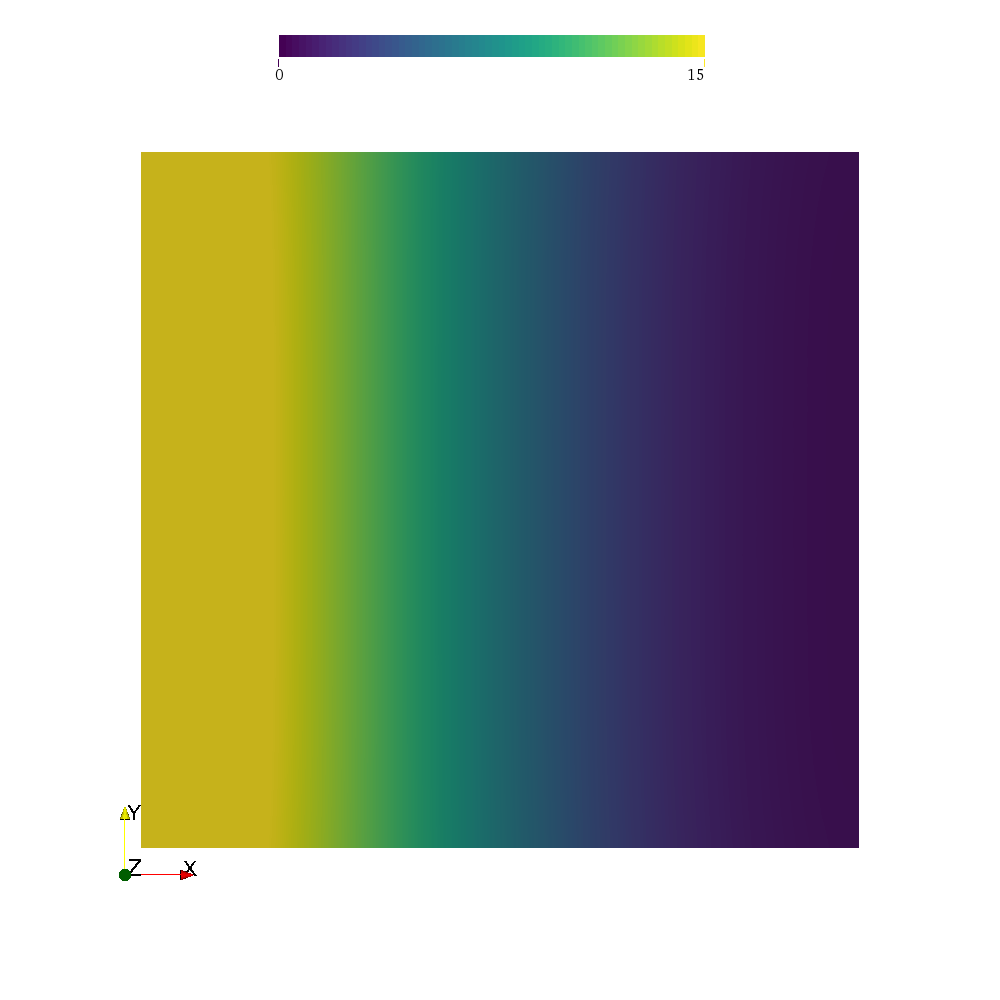
\includegraphics[height = 3 cm, trim = {6cm 6cm 6cm 6cm}, clip]{fig/Verificacion_Teorema/500h}
	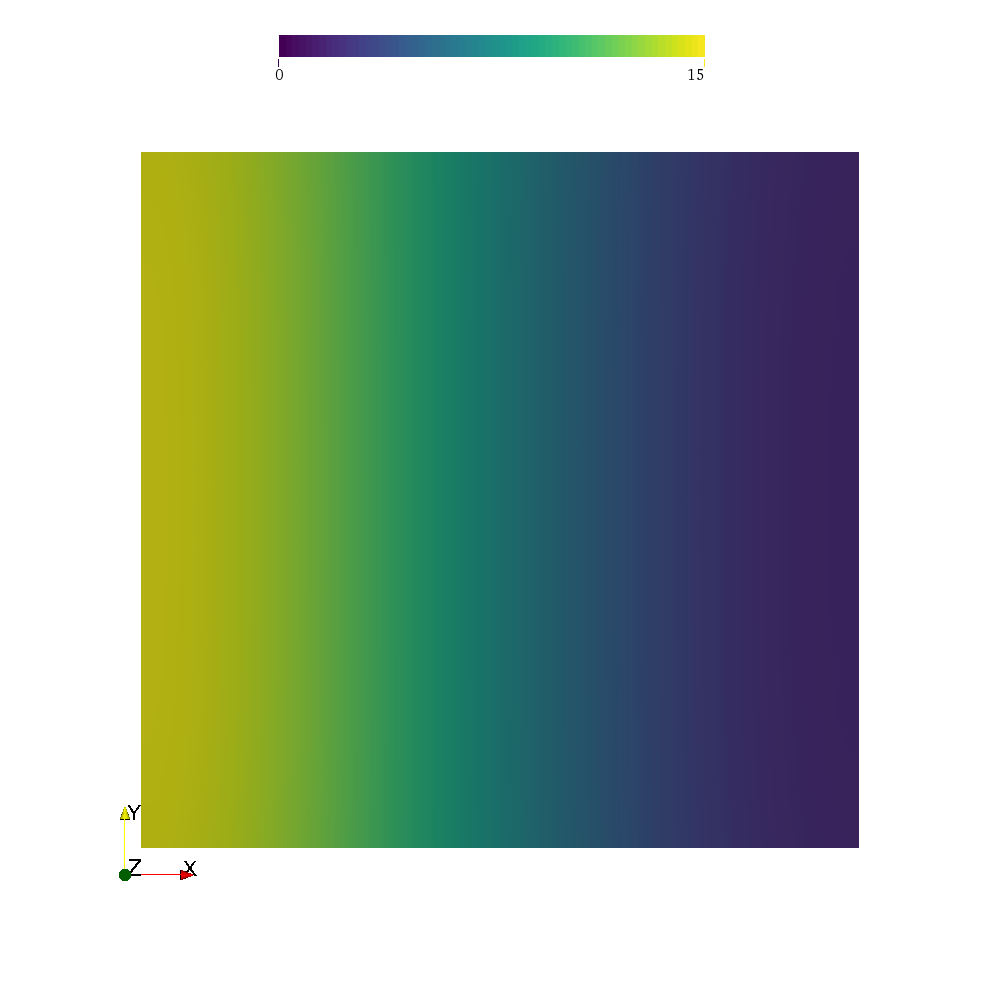
\includegraphics[height = 3 cm, trim = {6cm 6cm 6cm 6cm}, clip]{fig/Verificacion_Teorema/700h}\\[0.3 cm]
	
	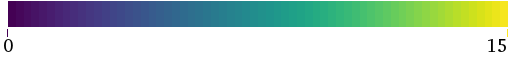
\includegraphics[height = 0.7 cm]{fig/Verificacion_Teorema/colourbar_diffusion}	
	\caption{Temporal evolution of the exact (up) and the homogenized (down) solution. From left to right we have $t = 20 ms$, $t = 250 ms$, $t = 500 ms$, $t = 700 ms$.} \label{fig:surrogate_ver}
\end{figure}

The evolution of both exact and homogenized solutions in time can be appreciated in figure \ref{fig:surrogate_ver}, and the error time evolution is in figure \ref{fig:verification_error_L2}. The error decrease in time, as is expected. Also, it can be noted that the error is greater when $\nabla \phi$ is greater, as is expected too, because the diffusion term is homogenized only. So, if diffusion decreases then L2$-$error also decreases.

This example is a worst-case-scenario, because the collagen inclusions are huge. In fact, from a physiological point of view, the values of $\theta_c$ and $\theta_f$ describes a very fibrotic tissue.


It has to be noted that the conduction velocity (CV) is a little bit underestimated in the homogenized model. This is due to the existence of paths without collagen in the mesh for exact problem, i.e., there are some ways where the potential propagates withouth any obstacles, and this is not considered by the effective tensor. Nevertheless, the difference is small, and the behavior of homogenized solution is well enough to reproduce the potential reaction-diffusion, as we will see in the section of numerical experiments.

The finite element method was implemented by using the FEniCS \cite{FENICS} open source library, which is composed of DOLFIN, FFC, UFL, FIAT and UFC. The mesh was generated using the open-source program GMSH \cite{GMSH}. Both, FEniCS and GMSH were interfaced with Python codes.


\begin{figure}[!htb]
	\centering
	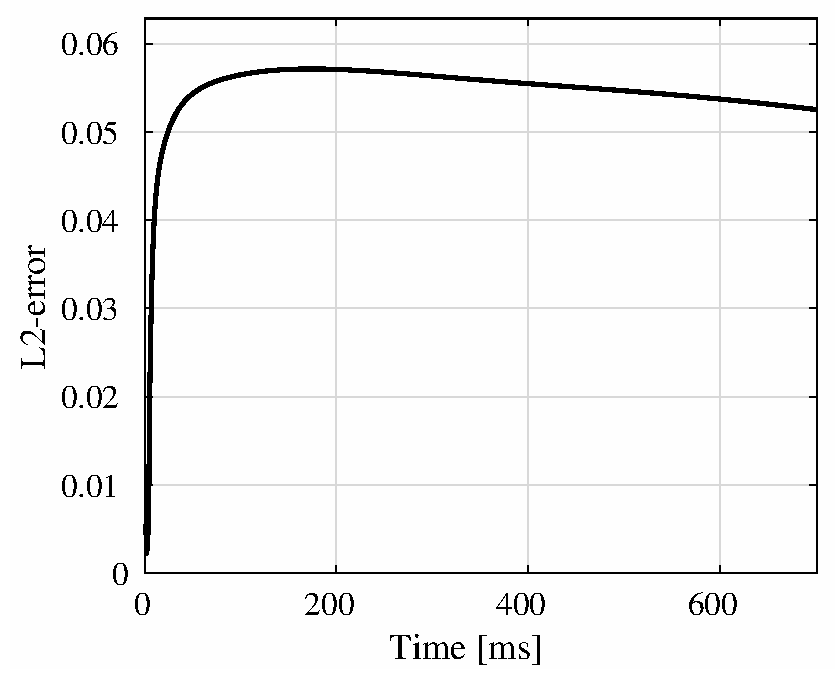
\includegraphics[height = 5 cm]{fig/Verificacion_Teorema/error_L2}
	\caption{Temporal evolution of L2-error for diffusion simulation.} \label{fig:verification_error_L2}
\end{figure}


\subsection{Discretization of the Minimal model}

The time discretization of the gating variables is semi-implicit. So first, for each time-step, the ODE's in \eqref{eq:mde_min} are solved using:


\begin{equation}
\arraycolsep=1.4pt\def\arraystretch{2.8}
\begin{array}{l}
r^{n+1} = \dfrac{r^n + (\Delta t r_{\infty}(1 - H(\phi - \theta_r)))/\tau_r^-}{1  +  (\Delta t (1 - H(\phi^n - \theta_r)))/\tau_r^- + (\Delta t H(\phi^n - \theta_r))/\tau_r^+} \\

w^{n+1} = \dfrac{w^n + (\Delta t w_{\infty}(1 - H(\phi - \theta_w)))/\tau_w^-}{1  +  (\Delta t (1 - H(\phi^n - \theta_w)))/\tau_w^- + (\Delta t H(\phi^n - \theta_w))/\tau_w^+} \\
   
s^{n+1} = \dfrac{s^n + \Delta t (1 + tanh(k_s (\phi^n - \phi_s)))/(2 \tau_s)}{(1 + \Delta t / \tau_s)}
\end{array}  \label{eq:mono_disc_gating}
\end{equation}

whose solutions are plugged in the PDE:

\begin{equation}
\dfrac{\phi^{n + 1} - \phi^n}{\Delta t}=  div(D \nabla \phi^{n+1}) - (J_{fi}^n + +  J_{si}^n + J_{so}^n) \label{eq:mono_disc_phi}
\end{equation}

The idea is to solve a stationary problem for each time step. This will be achieved trough a finite element method. 

Since we gonna use only Neumman boundary conditions for the numerical experiments, let us consider the test function space $V = \{ v \in H^1(\Omega) \}$. Multiplying \eqref{eq:mono_disc_phi} by a function of this space, integrating over all $\Omega$, considering the no-flux boundary conditions, and remembering the Green's Theorem, the weak form of the partial differential equation is obtained, so the problem can be re-written in the form $a (\phi^{n+1}, v) = L (v)$ as follows:

\begin{align}
a (\phi, v) = & \int_{\Omega} \phi v  d \Omega + \Delta t \int_{\Omega} D \nabla \phi \nabla v d \Omega \\
L (v) = & \int_{\Omega} \phi^n v d \Omega + \Delta t \int_{\Gamma_N} g v ds - \Delta t \int_{\Omega}( J_{fi}^n +  J_{si}^n + J_{so}^n )v d \Omega \label{eq:mde_min_weak}
\end{align}

where the notation $\phi = \phi^{n+1}$ is taken while there is no confusion in the meaning of the variables. Note that the currents are calculated using $\phi^n$, $r^{n+1}$, $w^{n+1}$ and $s^{n+1}$. 

Now, let us consider the finite dimensional space $V_h \subset V$ and the Galerkin method:

\begin{equation}
\phi = (c_1, c_2, ..., c_k) \cdot (\xi_1, \xi_2, ...., \xi_k) = \sum_{i=1}^k a_i \xi_i \label{eq:galerkin_method}
\end{equation}

where k is the total number of degrees of freedom, the functions $\{\xi_i \}_{i=1}^k$ belongs to the space $V_k$ and $c_i$ is the solution at the i-node. This way, the problem can be spatially discretized replacing \eqref{eq:galerkin_method} on equation \eqref{eq:mde_min_weak}. So, the problem is: find $\phi\in V$ such that $a_h (\phi, v) = L_h(v) \forall v\in V_h$, where 

\begin{align*}
a_h = & \int_{\Omega} (c_1, c_2, ..., c_k) (\xi_1, \xi_2, ...., \xi_k) \cdot (\xi_1, \xi_2, ...., \xi_k) ~ d \Omega \\
& + \Delta t \int_{\Omega} D (c_1, c_2, ..., c_k) (\nabla \xi_1, \nabla \xi_2, ...., \nabla \xi_k) \cdot (\nabla \xi_1, \nabla \xi_2, ...., \nabla \xi_k)~ d \Omega \\
L_h = & \int_{\Omega} (c_1^n, c_2^n, ..., c_k^n) (\xi_1, \xi_2, ...., \xi_k) \cdot (\xi_1, \xi_2, ...., \xi_k)~ d \Omega \\
& - \Delta t \int_{\Omega} (\gamma_1, \gamma_2, ..., \gamma_k) (\xi_1, \xi_2, ...., \xi_k) \cdot (\xi_1, \xi_2, ...., \xi_k)~ d \Omega
\end{align*}



where the test functions were discretized with $V_h$ functions. The current $J^n = J_{so}^n + J_{si}^n + J_{fi}^n$ was also discretized using $J = \sum_{i=1}^k \gamma_i \xi_i$. Now, defining the usually called \textsl{mass matrix}  $M \in \mathbb{M}_{k \times k}; M_{ij} = \int \xi_i \xi_j d \Omega $ and the \textsl{stifness matrix} $K \in \mathbb{M}_{k \times k}; K_{ij} = \int (D \nabla \xi_i) \cdot \nabla \xi_j d \Omega$, the discretized weak form yields to:

\begin{equation}
(M + \Delta t K) c^{n+1} = M c^n - \Delta t M \vec{\gamma} \label{eq:Ax=b}
\end{equation}

where $c^{n+1} = (c_1, c_2, ..., c_n)$ and $c^n = (c_1^n, c_2^n, ..., c_k^n)$. Finally, the space $V_h$ is chosen as the set of piecewise linear functions over each element.

The update of the \textsl{rhs} vector $(M c^n - \Delta t M \vec{\gamma})$ is done at each time-step, while the matrix $(M + \Delta t K)$ is just assembled once at the start of the simulation. Finally, we solve the linear system by using the conjugate gradient method. Also, in order to improve the convergence of the iterative method, an AMG preconditioner is applied before solving the linear system.


\subsection{Discretization of the FHN model}

The FitzHugh-Nagumo model can be plugged in the Monodomain equation \eqref{eq:MDE}, obtaining:  

\begin{equation}
\arraycolsep=2.5pt\def\arraystretch{2.8}
\begin{array}{rl}
\dfrac{\partial \phi}{ \partial t} = & div(D \nabla \phi) + c_1 \phi (\phi - \alpha)(1 - \phi) - c_2 w \\ 
\dfrac{\partial w}{\partial t} = & c_2 (\phi - wd)\\
\end{array}
 \label{eq:MONO+FHN}
\end{equation}

In order to better understand the numerical behavior of the problem, a stability analysis is performed in the following paragraphs.

\subsubsection{Stability Analysis}

The system \eqref{eq:MONO+FHN} is equivalent to:

\begin{equation} 
\phi \dfrac{\partial \phi}{ \partial t}  = \{ c_1 \phi (\phi - \alpha)(1 - \phi) - c_2 r \}\phi
\end{equation}

\begin{equation}
r \dfrac{\partial r}{\partial t}  = \{ c_2 (\phi - rd) \} r
\end{equation}

Now, adding both equations and defining E as:
\begin{equation}
\phi \dfrac{\partial \phi}{ \partial t} + r \dfrac{\partial r}{\partial t} = \frac{1}{2} \frac{d}{dt} \left(\phi^2 + r^2 \right):= E
\end{equation}

we obtain:

\begin{equation}
E = c_1 (1 + \alpha) \phi^3 - c_1 (\alpha \phi^2 +  \phi^4) -c_2 d r^2 \label{eq:total_energy}
\end{equation}

where the coupling term $c_2 \phi r$ has been canceledd. The E magnitude can be interpreted as the total energy of the system. In this context, results natural the anulation of the coupling term, since the energy cannot be generated in the ``interface'' of the system. Note that nearly all terms in the right side of equation (\ref{eq:total_energy}) dissipates energy from the system, in exception of $c_1 (1 + \alpha) \phi^3$, that constitutes a potential instability source. So, the balance between this last and the others terms conditions the decay of the solution.

Its desirable that the discretized version of the  system preserves the stability properties of the continuous system. To evaluate this, a general $\theta-$scheme can be used for the time discretization of the EDO, while a ``$\beta-$scheme'' can be used for the PDE, where the discretization has been done in order to obtain a linear problem:

\begin{equation}
\arraycolsep=1.4pt\def\arraystretch{2.2}
\begin{array}{rl}
\dfrac{r^{n+1}-r^n}{\Delta t} 
= &\{ \beta (c_2 \phi^{n + 1}) + (1 - \beta  )(c_2 \phi^{n + 1}) \} 
- \{ \theta  (c_2 d r^{n + 1}) + (1 - \theta )c_2 d r^{n} \} \\

\dfrac{\phi^{n+1} - \phi^n}{\Delta t}
= &c_1(1 + \alpha)\phi^n \{ \beta (\phi^{n+1})^2 + (1 - \beta) (\phi^{n})^2 \} 
- c_1 \alpha \{ \beta \phi^{n+1}  + (1 - \beta) \phi^n \} \\
&- c_1 (\phi^n)^2 \{ \beta \phi^{n+1} \} 
 - c_2 \{\theta r^{n+1} + (1 - \theta) r^{n} \}
\end{array} \label{eq:teta_esquema_MDE}
\end{equation}

where $\phi^{n}$ and $r^{n}$ are the potential and internal variable at the time step n, respectively. There exist, for instance, the following cases:

\begin{itemize}
\item $\theta = \beta = 0 \rightarrow$  explicit (forward Euler) and uncoupled problem.
\item $\theta = 1$ and $\beta = 1 \rightarrow$ implicit (backward Euler) and coupled problem.
\item $\theta = 1/2$ and $\beta = 1/2 \rightarrow$ implicit (Crank-Nicolson) and coupled problem.  
\end{itemize}

In general, for $\beta$ and $\theta$ greater than a half, implicit schemes will be obtained. To understand the energy change of the discrete system in time the equations (\ref{eq:teta_esquema_MDE}) are multiplied by $r^{n + \theta}$ and $\phi^{n + \beta}$ up and down, respectively, were the notation $a^{n + \theta} := \theta a^{n+1} + (1 - \theta), a^n$ has been adopted. Now, after some algebra arrangements the following is obtained:

\begin{equation}
\arraycolsep=1.4pt\def\arraystretch{2.2}
\begin{array}{llr}
\overline{E}:= & \dfrac{1}{2} \dfrac{r^{n+1}}{dt} - \dfrac{1}{2} \dfrac{r^{n}}{dt} + \dfrac{1}{2} \dfrac{\phi^{n+1}}{\Delta t} - \dfrac{1}{2} \dfrac{\phi^{n}}{\Delta t} \\

& = c_2 \phi^{n + \beta} r^{n + \theta} 
- c_2 d (r^{n + \theta})^2 
- \red{(\theta - \frac{1}{2}) \frac{1}{\Delta t} (r^{n+1} - r^n)^2} 
+ c_1 (1 + \alpha) \phi^n (\phi^{n + \beta})^2 \\
& - c_1 \alpha (\phi^{n + \beta})^{2}
- c_1 (\phi^n)^2 (\phi^{n + \beta})^2
- c_2 r^{n + \theta} v^{n + \beta}
- \red{(\beta - \frac{1}{2}) \frac{1}{\Delta t} (\phi^{n+1} - \phi^n)^2 }
\end{array}
\end{equation}

where $\overline{E}$ is the total ``\textsl{numerical energy}'' of the system. Note that the terms in red are not present in the continuos stability analisys, so is desirable, in order to preserve stability properties of the continuous system, that this term does not add energy to the system, is achieved simply by considering $\theta \geqslant 0.5$ and $\beta \geqslant 0.5$.

Finally, the following \textsl{semi-implicit} squeme is adopted:

\begin{equation}
\arraycolsep=1.4pt\def\arraystretch{2.2}
\begin{array}{llr}
\dfrac{r^{n+1} - r^n}{\Delta t} = c_2 \phi^n - c_2 d r^{n+1} \\
\dfrac{\phi^{n+1} - \phi^n}{\Delta t} = c_1 (1 + \alpha) (\phi^n)^2 - c_1 \alpha \phi^{n+1} - c_1 (\phi^n)^3 + div(D \nabla \phi^{n+1})
\end{array} \label{eq:FHN_semi_imp}
\end{equation}

where all the non-linear terms has been left explicit, and the linear ones has been left implicit. Also, the potential in the internal FHN equation has been left explicit, in order to finally obtain a linear and uncoupled problem. Note that the diffusion term has been added and was left implicit, in order to circunvent the well-knowed stability issues of a explicit diffusion term.

\subsubsection{Weak Form}

The weak variational form of the time-discretized PDE must to be written in order to perform a FEM discretization of the space. The variational form at each time step $n$ is $a(\phi^{n + 1}, v) = L(v)$ 

\begin{equation}
\arraycolsep=1.4pt\def\arraystretch{3}
\begin{array}{rcl}
a (\phi^{n + 1}, v)& = & \displaystyle \int_{\Omega} (1 + \Delta t c_1 \alpha) \phi^{n+1} v ~d \Omega + \Delta t \int_{\Omega} D \nabla \phi^{n+1} \nabla v ~d \Omega \\
L(v)& = &\displaystyle \int_{\Omega} \phi^n v ~d \Omega + \Delta t \int_\Omega \{ c_1(1 + \alpha)(\phi^n)^2 - c_1 (\phi^n)^3 - c_2 r^{n+1} \} v~ d \Omega + \Delta t \int_{\Gamma_N} g  v ~ds 
\end{array} \label{eq:esquema_definitivo}
\end{equation}


Now we can solve the problem by first solving the internal gatting variable equation and then solving \eqref{eq:esquema_definitivo}

\subsection{Experiment \# 1: Single Cell}

\subsubsection{Results Using FHN Reaction Model:}


First, a case with a small domain can be simulated, where the spatial dependence can be neglected (single cell). In figure \ref{fig:fhn_nofisiologico2} we can see the solution in time. As initial conditions we take $\phi(0) = 0.2 [mV]$ and $r(0) = 0$. The time step is $1 [ms]$. 

\begin{figure}[H]
\centering 
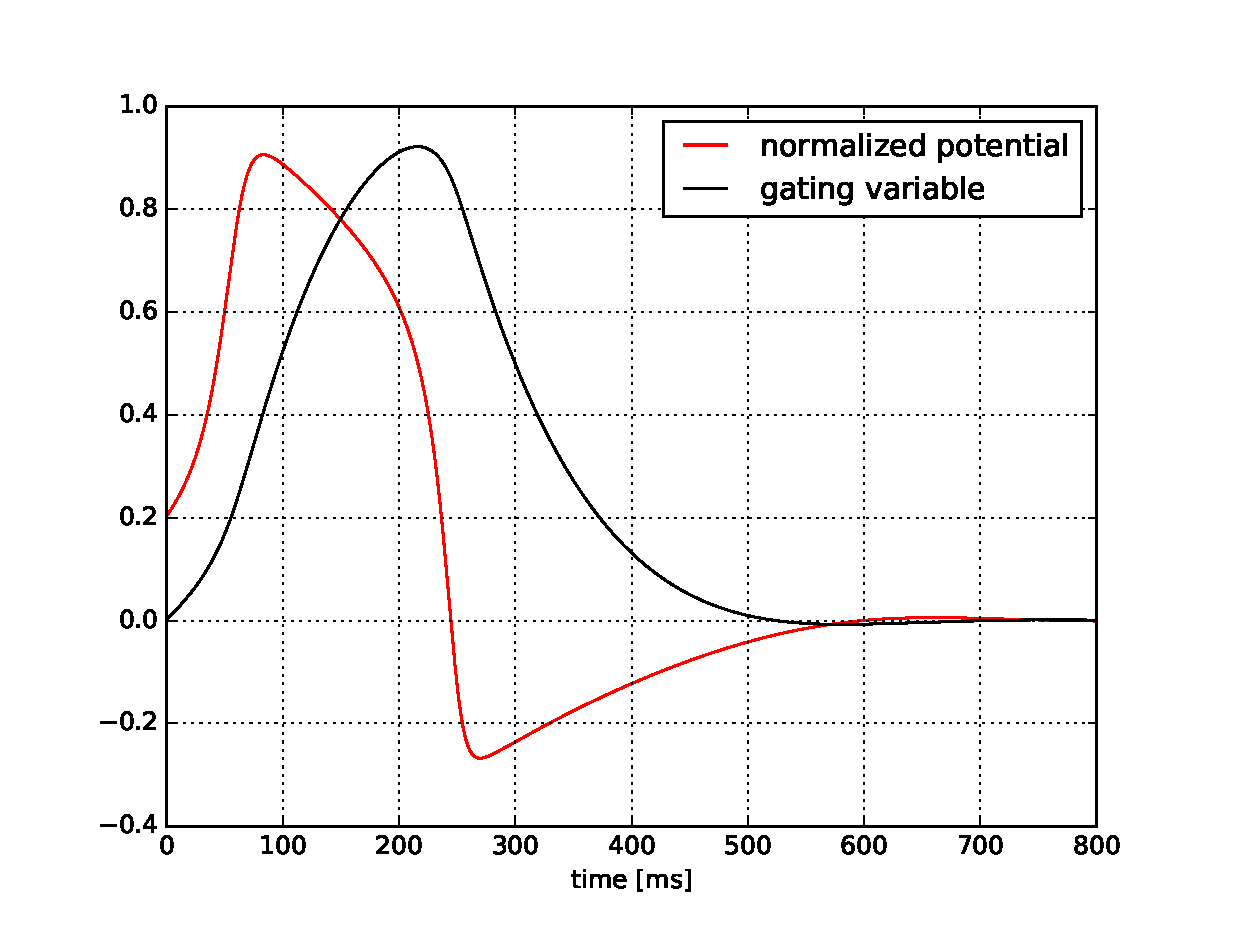
\includegraphics[height = 6 cm]{fig/Numerical_Experiments/ex1/EX1-FHN_single_cell.eps}
\caption{numerical solution of the FitzHugh-Namuno equations.}
\label{fig:fhn_nofisiologico2}
\end{figure}

The parameters used to generate the results can be appreciated in the table \ref{tab:parametros_FHN}.

\begin{table}[!htbp]
\centering
\caption{ Parameters used in the simulation.}
\label{tab:parametros_FHN}
\begin{tabular}{@{}cccc@{}}
\toprule
Parameter & Description                    & Value & Units  \\ \midrule
$c_1$     & Excitation rate constant       & 0.175 & $1/ms$ \\
$c_2$     & Excitation decay constant      & 0.03  & $1/ms$ \\
b         & Recovery rate constant         & 0.011 & $1/ms$ \\
d         & Recovery decay constant        & 0.55  & -      \\
$\alpha$  & Normalized threshold potential & 0.08  & -      \\ \bottomrule
\end{tabular}
\end{table}
Other approaches closer to the fully implicit discretization were tested, in order to see how far the time-step can be reduced. Nevertheless, the difference is negligible ($\approx 0.5 ~[ms]$), so the use of other schemes was discarded, because is preferable to have a positive definite system with a little bit lower time-step than a non positive definitive system with a negligible gain in the time step. On the other hand, with a fully implicit scheme it was noted that the time step can be severely increased (nearly 18 times the semi-implicit value), but this approach is also not considered because the system becomes highly computational expensive.

\subsubsection{Results Using Minimal Reaction Model:}

We solve the equations \eqref{eq:mono_disc_phi} and \eqref{eq:mono_disc_gating} over a small domain using the Minimal model for the reaction term. The dimensionless voltage variable is re-scaled to obtain values inside the physiological range by using the equation $\phi_{mV} = 85.7 \phi - 84$ or $\phi_{mV} = 85.7 \phi - 80.9$ if the tissue belongs to the atrial chamber. Initial scaled conditions are $\phi = 0$, $r = 1$, $w = 1$ and $s = 0$. A stimulus of $52 [mV]$ is applied for $0.2 [ms]$, in order to reproduce the $Na^+$ channels overture, i.e., the transition to phase 1. Note that this value is over the threshold needed to generate the cells action potential. A time-step of $0.1 [ms]$ is used. The result of the implementation can be seen in the figure \ref{fig:mde_min_ex1_single-cell}.

\begin{figure}[!htbp]
	\centering
	\subfigure[epicardial cell.]{
		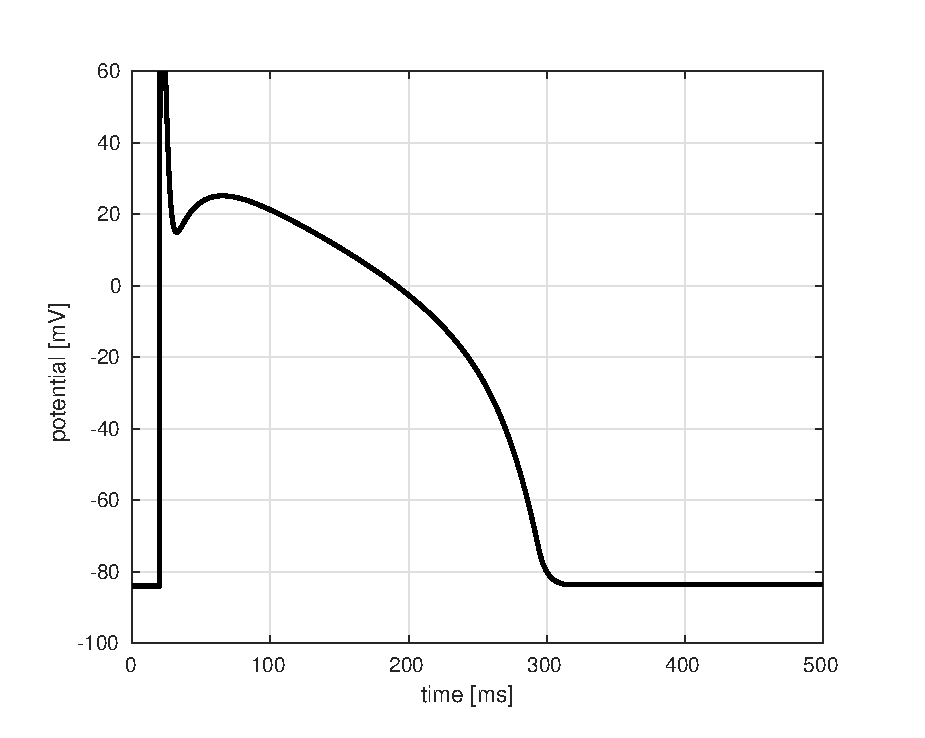
\includegraphics[width = 5 cm]{fig/Numerical_Experiments/ex1/ex1_min_epi}}
	\subfigure[endocardial cell.]{
		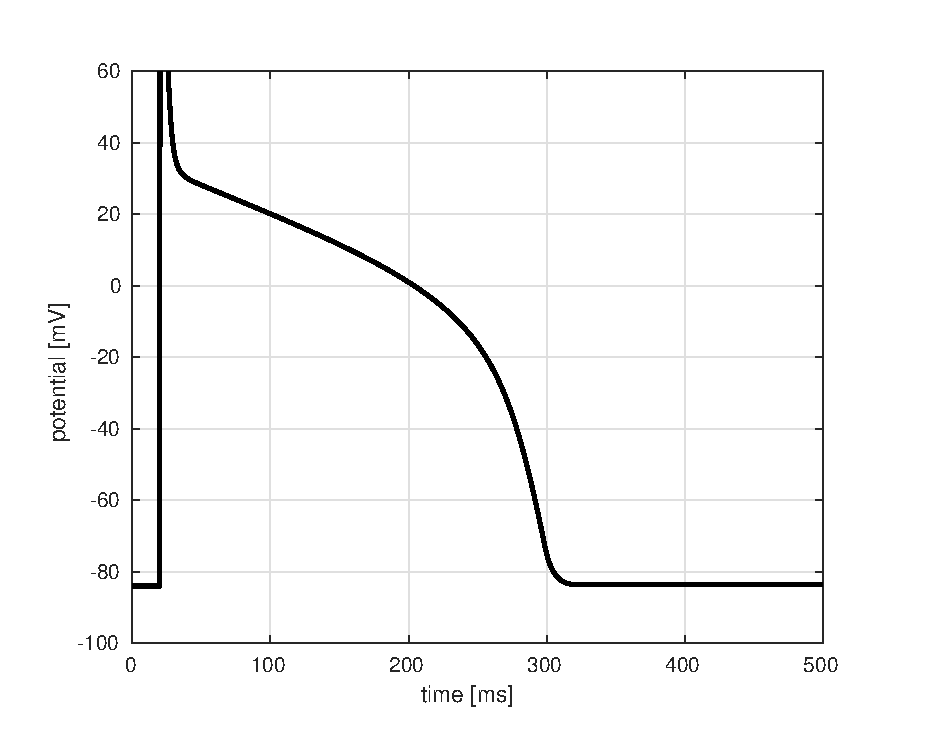
\includegraphics[width = 5 cm]{fig/Numerical_Experiments/ex1/ex1_min_endo}}
	\subfigure[mid-myocardial cell.]{
		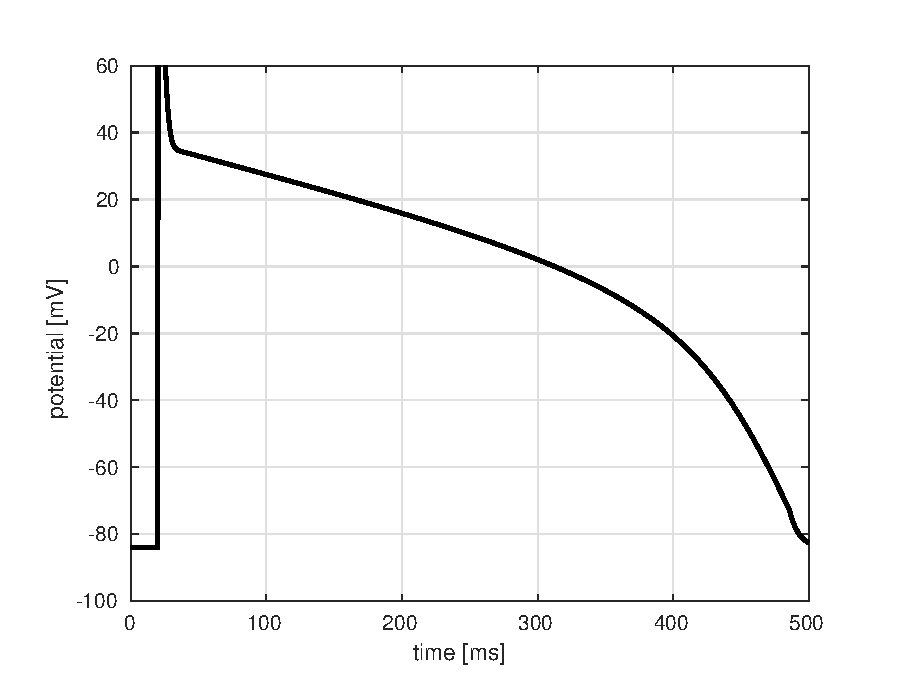
\includegraphics[width = 5 cm]{fig/Numerical_Experiments/ex1/ex1_min_mid}}
	\subfigure[atrial cell.]{
		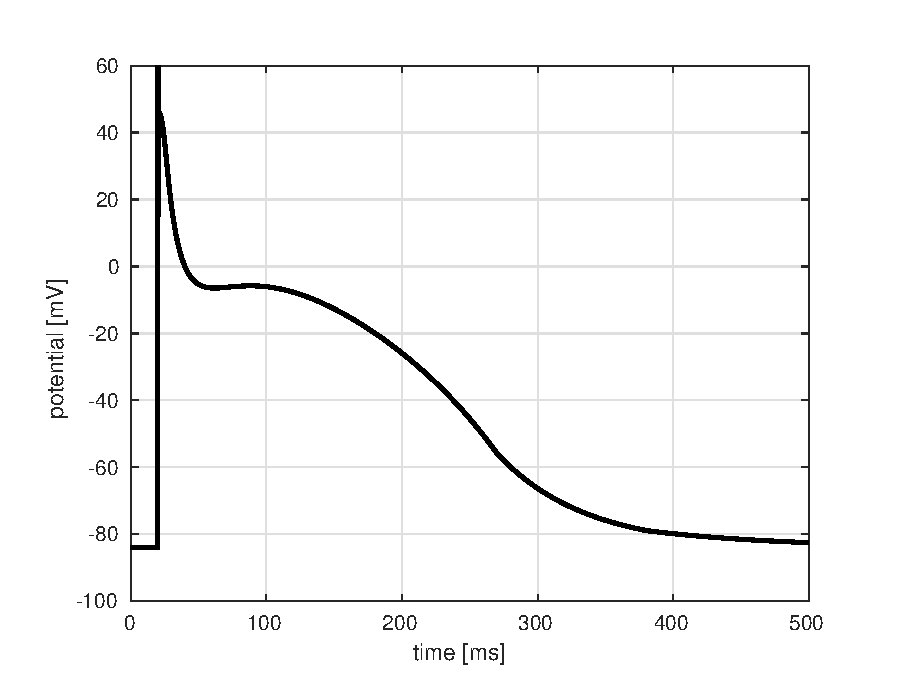
\includegraphics[width = 5 cm]{fig/Numerical_Experiments/ex1/ex1_min_atrial}}
	\caption{Simulated human AP for different configurations.} \label{fig:mde_min_ex1_single-cell}
\end{figure}	

If we look at the figures \ref{fig:fhn_nofisiologico2} and \ref{fig:mde_min_ex1_single-cell} we can observe the different advantages of the minimal model over the FHN: AP duration and shape are more realistic in the Minimal model and emulates better the refractory time, because by construction of the reaction model, the cell will can not repolarizate if is in phase 0, phase1, phase 2 or the beginning of phase 3. On the other hand, the FHN model is cheaper regards to computational cost but not enough to considerate FHN over Minimal. 

\subsection{Experiment \# 2: Tissue with High Fibrosis}

On this simulation we consider a cardiac tissue with high level of diffuse fibrosis. Both problems, exact and homogenized (surrogate model) will be compared. 

The geometry is a two dimensional $25 \times 25~mm^2$ square. A normalized stimulus of 1.587 for Minimal and 1.0 for FHN is applied in the left boundary during the first three seconds of the simulation. 

\subsubsection{Results Using FHN Cell Model:}

In the figure \ref{fig:ex2FHN} we can see the results of the simulations using the FHN reaction model, with the parameters of the table \ref{tab:parametros_FHN}. The potential is scaled to physiological range by using $\phi_{mv} = 110 \phi - 80$. The time step is $\Delta t = 0.5~[ms]$. The L2$-$error evolution with time is presented in figure \ref{fig:ex2_errorFHN}.

\begin{figure}[!htbp]
	\centering
	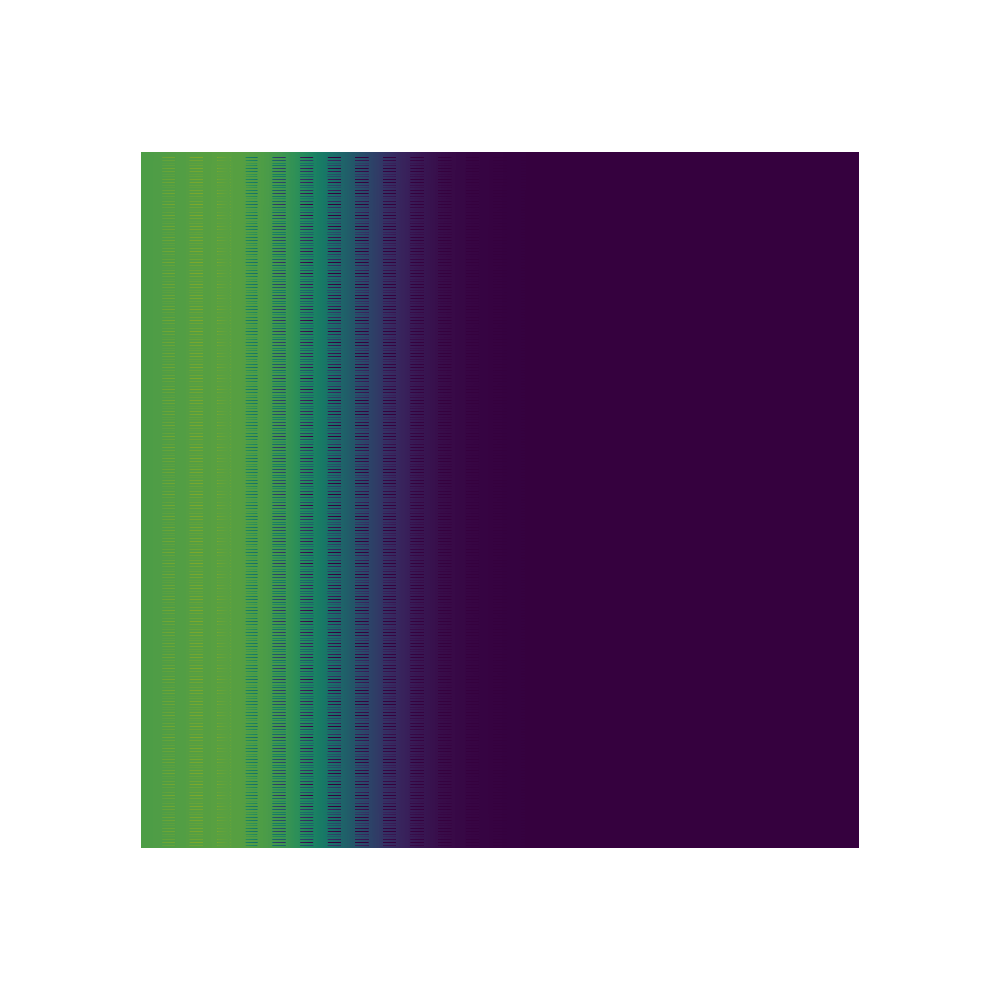
\includegraphics[height = 3 cm, trim = {6cm 6cm 6cm 6cm}, clip]{fig/Numerical_Experiments/ex2/FHN/100}
	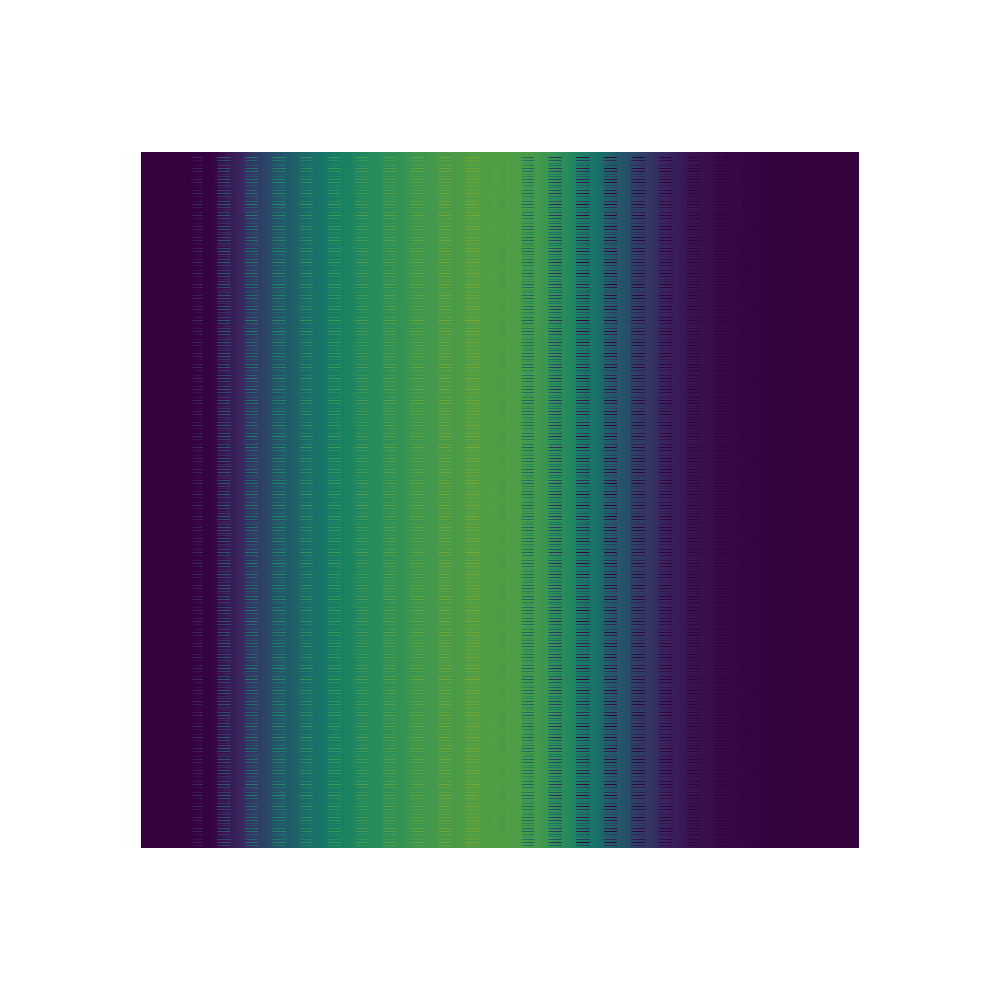
\includegraphics[height = 3 cm, trim = {6cm 6cm 6cm 6cm}, clip]{fig/Numerical_Experiments/ex2/FHN/250}
	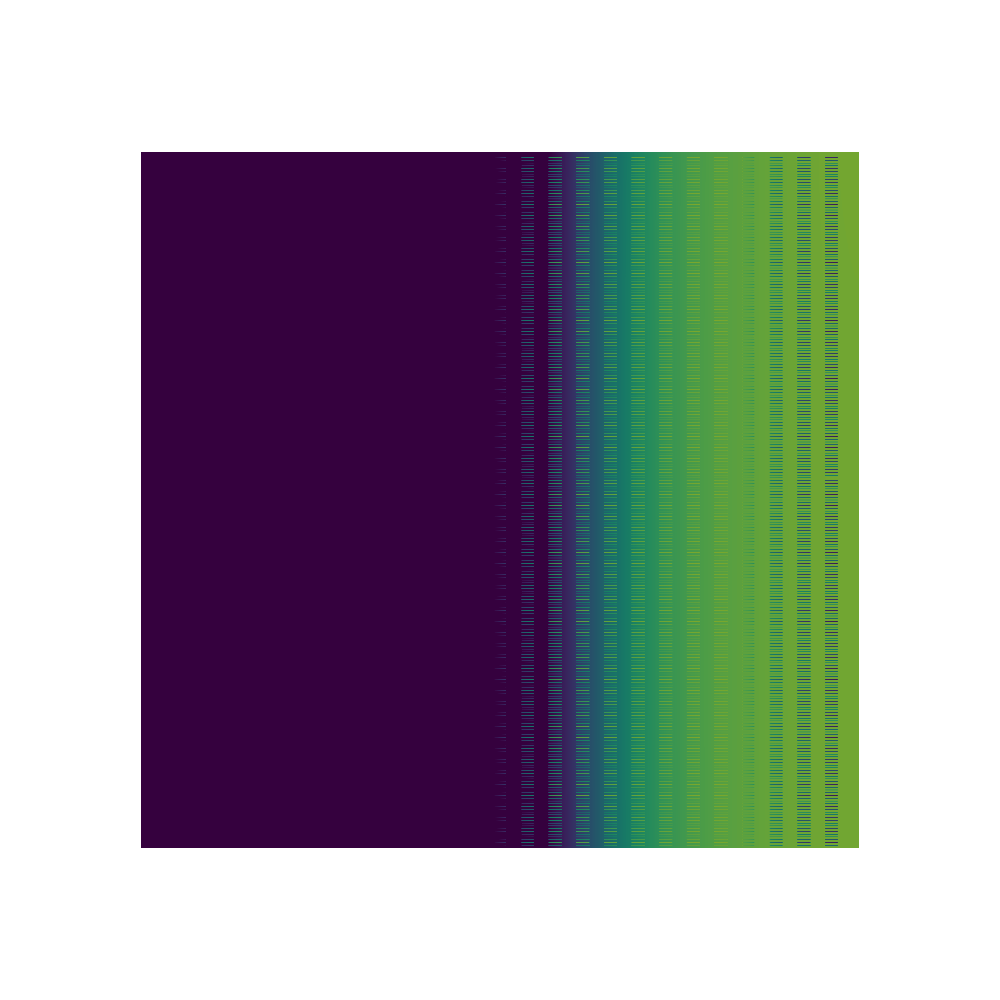
\includegraphics[height = 3 cm, trim = {6cm 6cm 6cm 6cm}, clip]{fig/Numerical_Experiments/ex2/FHN/390} \\
	
\includegraphics[height = 3 cm, trim = {6cm 6cm 6cm 6cm}, clip]{fig/Numerical_Experiments/ex2/FHN/100h}
	
\includegraphics[height = 3 cm, trim = {6cm 6cm 6cm 6cm}, clip]{fig/Numerical_Experiments/ex2/FHN/250h}
	
\includegraphics[height = 3 cm, trim = {6cm 6cm 6cm 6cm}, clip]{fig/Numerical_Experiments/ex2/FHN/390h} \\[0.3 cm]
	
	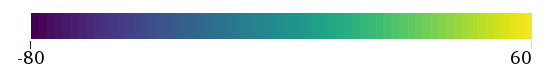
\includegraphics[height = 0.9 cm]{fig/Numerical_Experiments/colourbar_FHN}	
	\caption{temporal evolution of the exact (up) and the homogenized (down) solution. From left to right we have $t = 100 ms$, $t = 250 ms$ and $t = 390 ms$} \label{fig:ex2FHN}
\end{figure}

\begin{figure}[H]
\centering
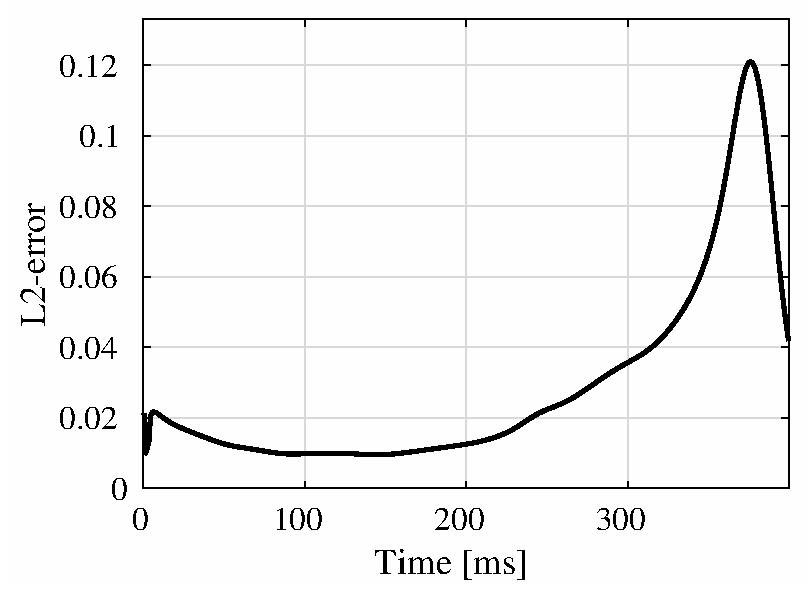
\includegraphics[height = 5 cm]{fig/Numerical_Experiments/ex2/FHN/error_L2}
\caption{L2-error evolution between exact and homogenized problem.} \label{fig:ex2_errorFHN}
\end{figure}

As can be appreciated, the surrogate models works good enough for the FHN reaction model from a macroscopic point of view.

\subsubsection{Results Using Minimal Gating Variables Model:}


In the figure \ref{fig:ex2Minimal} we can see the results of the simulations using the Minimal reaction model with atrial tissue parameters. The potential is scaled to physiological range by using $\phi_{mv} = 110 \phi - 80$. The time step is $\Delta t = 0.1~[ms]$. The results are presented in the figure \ref{fig:ex2Minimal}.

\begin{figure}[!htbp]
	\centering
	
\includegraphics[height = 3 cm, trim = {6cm 6cm 6cm 6cm}, clip]{fig/Numerical_Experiments/ex2/MINIMAL/3}
	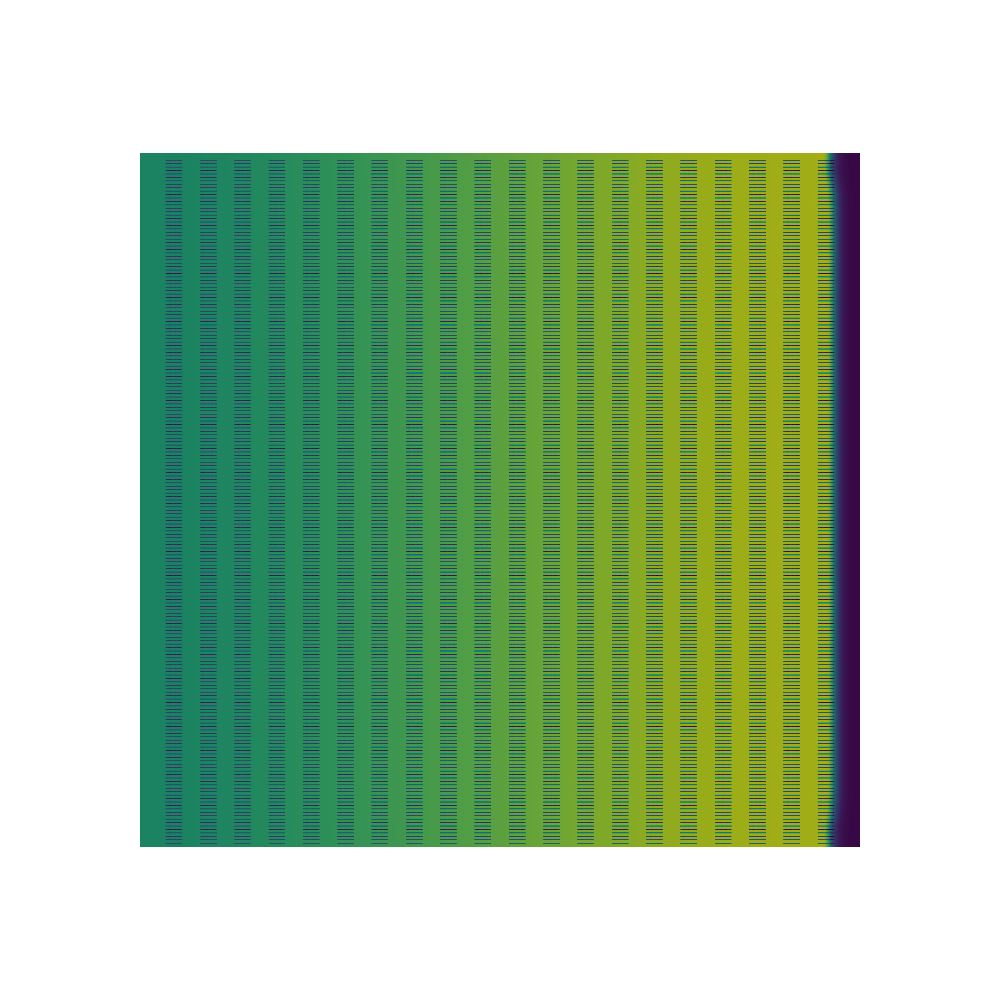
\includegraphics[height = 3 cm, trim = {6cm 6cm 6cm 6cm}, clip]{fig/Numerical_Experiments/ex2/MINIMAL/15}
	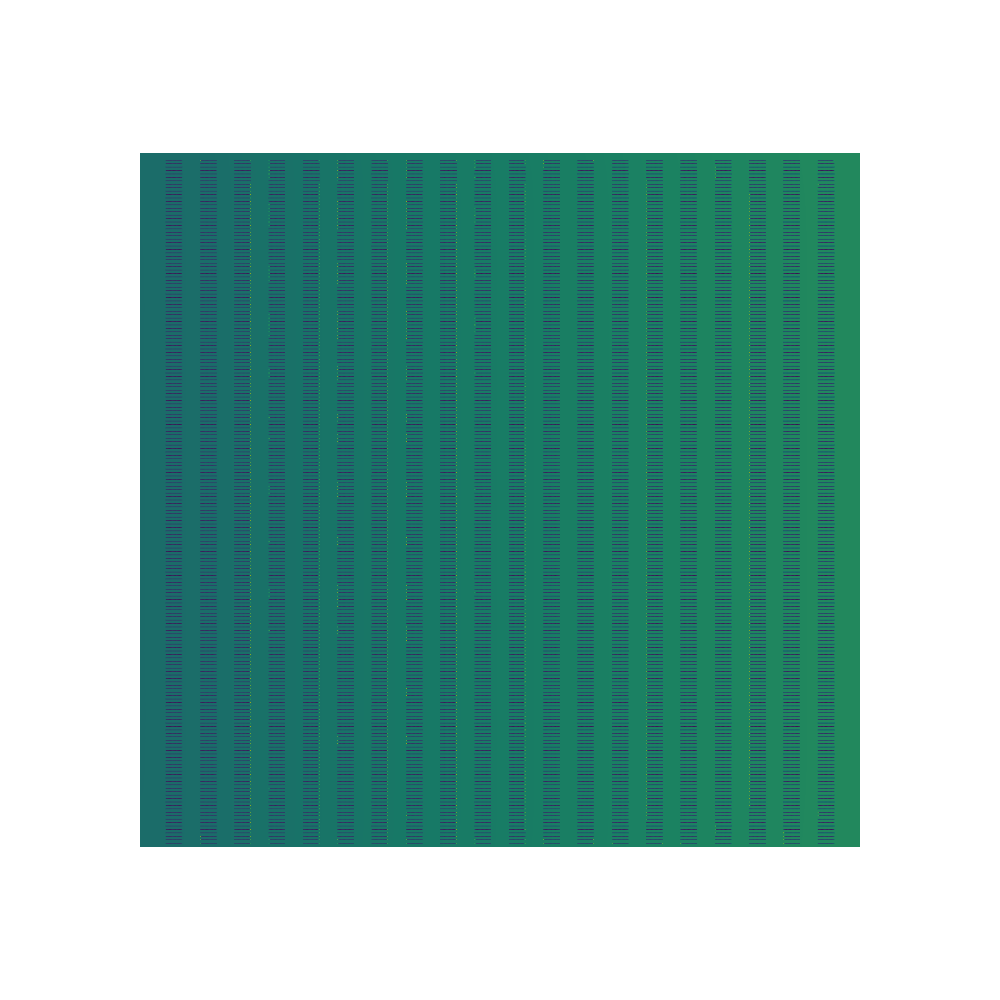
\includegraphics[height = 3 cm, trim = {6cm 6cm 6cm 6cm}, clip]{fig/Numerical_Experiments/ex2/MINIMAL/30} \\
	
\includegraphics[height = 3 cm, trim = {6cm 6cm 6cm 6cm}, clip]{fig/Numerical_Experiments/ex2/MINIMAL/3h}
	
\includegraphics[height = 3 cm, trim = {6cm 6cm 6cm 6cm}, clip]{fig/Numerical_Experiments/ex2/MINIMAL/15h}
	
\includegraphics[height = 3 cm, trim = {6cm 6cm 6cm 6cm}, clip]{fig/Numerical_Experiments/ex2/MINIMAL/30h}  \\[0.3 cm]
	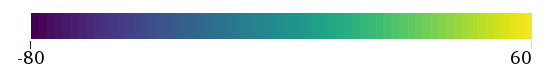
\includegraphics[height = 0.9 cm]{fig/Numerical_Experiments/colourbar_FHN}	
	\caption{Temporal evolution of the exact (up) and the homogenized (down) solution. From left to right we have $t = 3 ms$, $t = 250 ms$ and $t = 390 ms$} \label{fig:ex2Minimal}
\end{figure}


Note that the results are satisfactory, because the homogenized solution evolution reproduce the exact one in a mesoscopic scale, where interest of this study relays. The relative L2-error between both, the exact and homogenized solution, stay below totally acceptable values, as can be appreciated in figure \ref{fig:ex2_error}. 

\begin{figure}[!htbp]
	\centering
	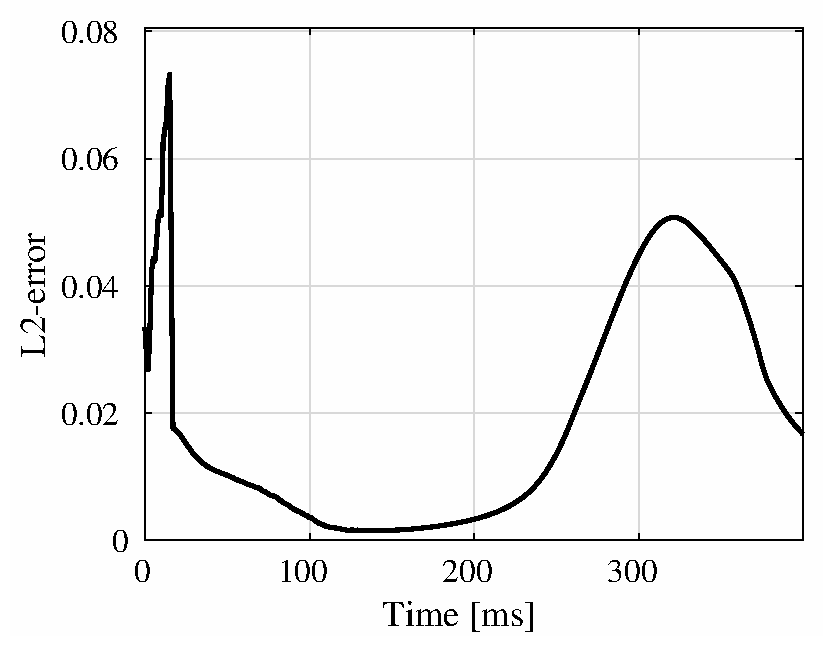
\includegraphics[height = 5 cm]{fig/Numerical_Experiments/ex2/MINIMAL/error_L2}
	\caption{L2-error evolution between exact and homogenized problem.} \label{fig:ex2_error}
\end{figure}

The first thing is to note how the front wave propagation is affected by the election of the reaction model. By inspection of the figures \ref{fig:ex2FHN} and \ref{fig:ex2Minimal} we can conclude that the front wave propagates faster in the minimal reaction model. Nevertheless, the mean behavior is quite similar in both FHN and Minimal models. A detailed view of the action potential for a cell located at the coordinates $(13~mm,~13~mm)$ is shown in the figure \ref{fig:cell_comparison}, where we can also note the difference between homogenized and exact problem. Furthermore, we can see how the surrogate model fits better with the exact solution when the Minimal reaction term is employed.

\begin{figure}[!htbp]
	\centering
	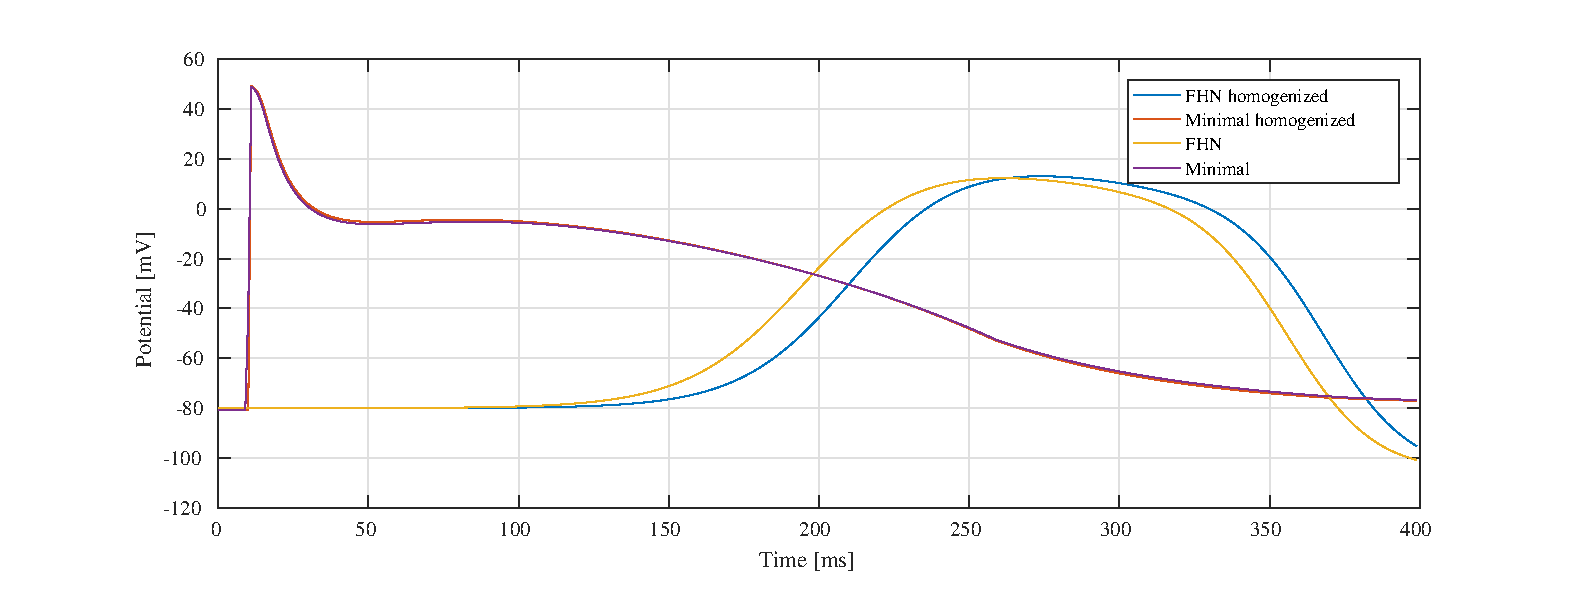
\includegraphics[height = 6.5 cm, trim ={2cm, 0cm, 0cm, 0cm}, clip]{fig/Numerical_Experiments/ex2/cell_comparison}
	\caption{Comparison of the action potential for a cell located at the coordinates $(13~mm,~13~mm).$}
	\label{fig:cell_comparison}
\end{figure}

\subsection{Experiment \# 3: Tissue with Stringy Fibrosis}

In this example the minimal model for mid-myocardial tissue will be used. Note that $\theta_c = 1$, so now there are vertical obstacles for the potential diffusion, as in figure \ref{fig:ex3_geo}. The reason to choose this configuration relays in impose a difficult case for the effective tensor. Characteristic mesh sizes are the same as previous examples.

\begin{figure}[!htbp]
\centering
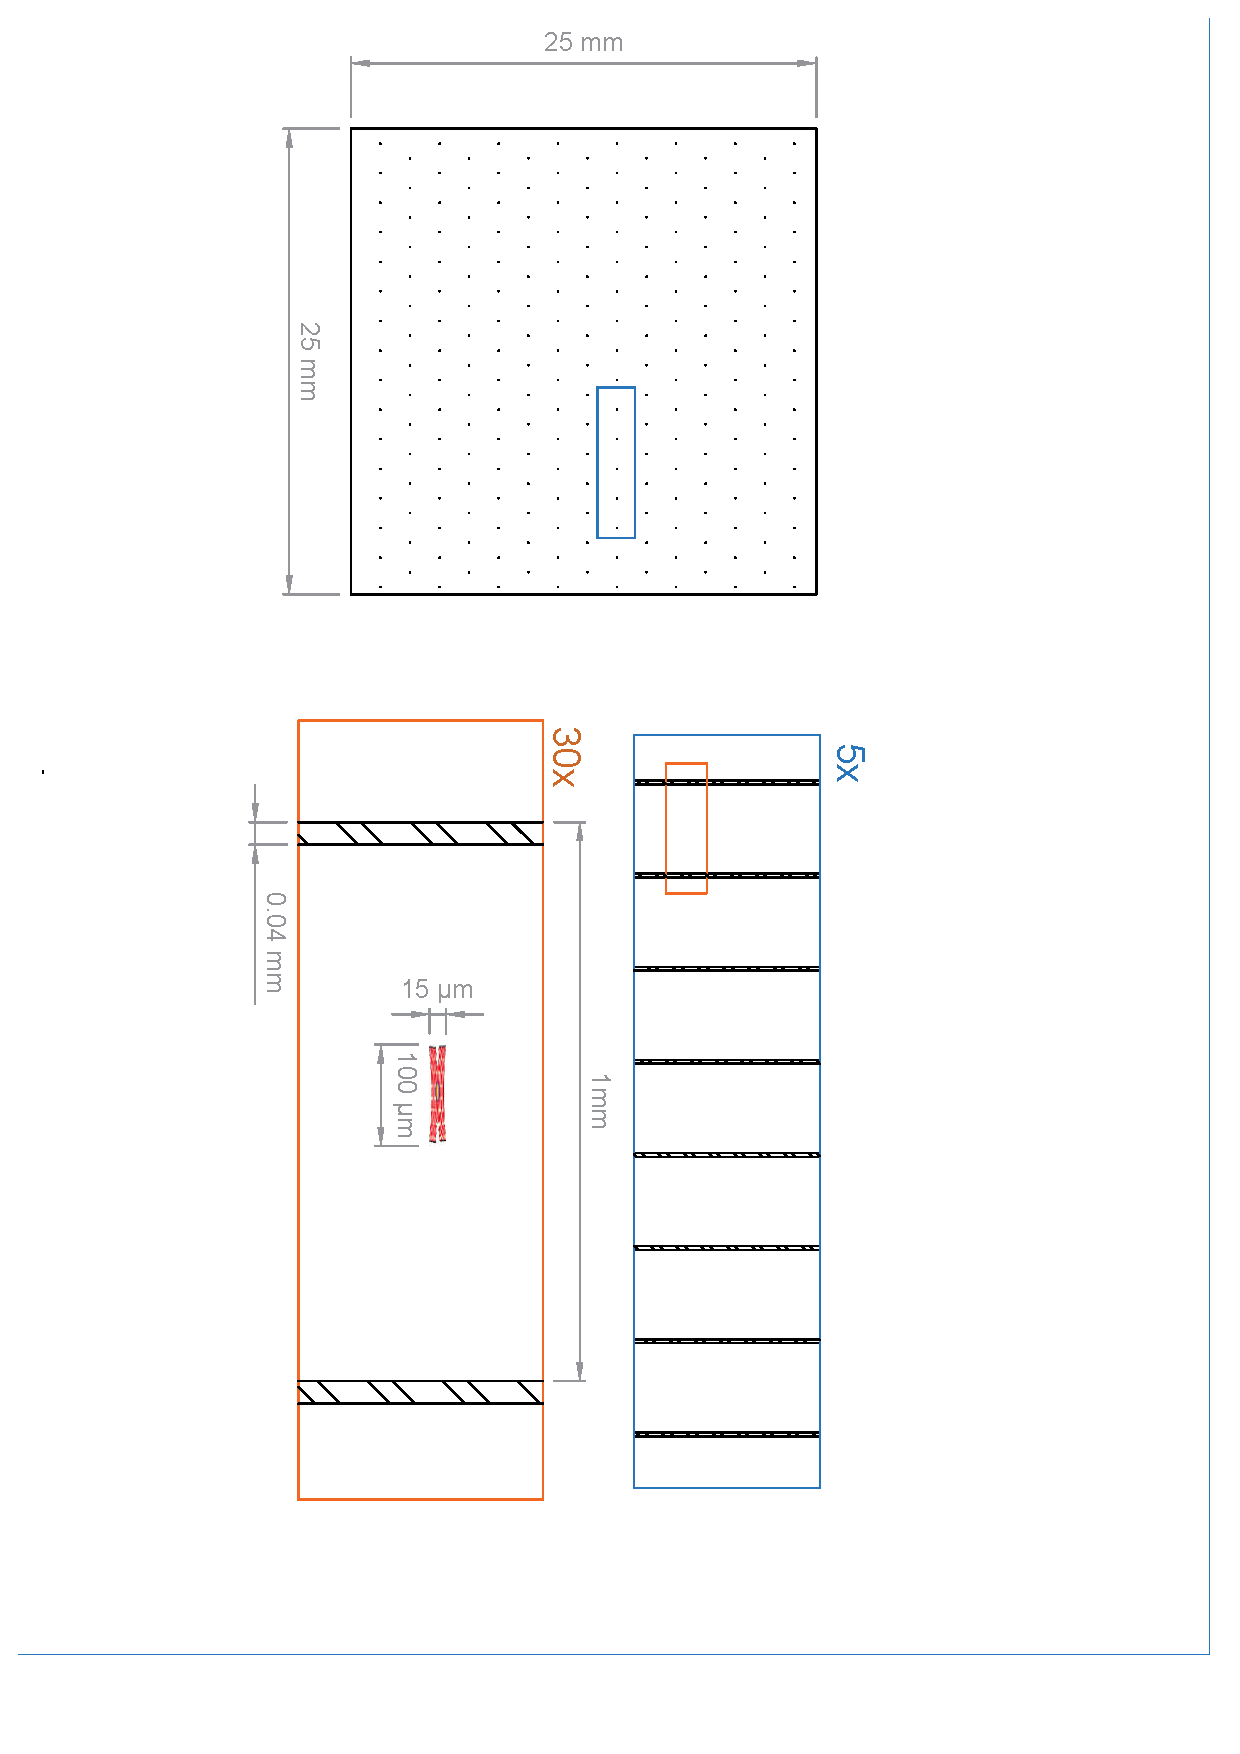
\includegraphics[trim={4.1cm 2cm 6cm 0.5cm}, clip, width = 6cm, angle = 90]{fig/Numerical_Experiments/ex3/geometry}
\caption{Geometry for example \# 3.} \label{fig:ex3_geo}
\end{figure}

The stimulus is applied at the right edge for 3 milliseconds, and has a intensity of $52~[mV/mm]$. $\theta_f$ is 0.04 and the time step is 0.1 milliseconds. For the initial conditions we pick $\phi = 0$, $r = 1$, $w = 1$ and $s = 0$. The implementation results are presented in figure \ref{fig:results_exp3}.

\begin{figure}[!htbp]
\centering
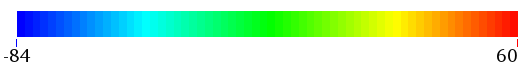
\includegraphics[height = 0.8 cm]{fig/Numerical_Experiments/ex3/ex3_colourbar}\\[0.1 cm]
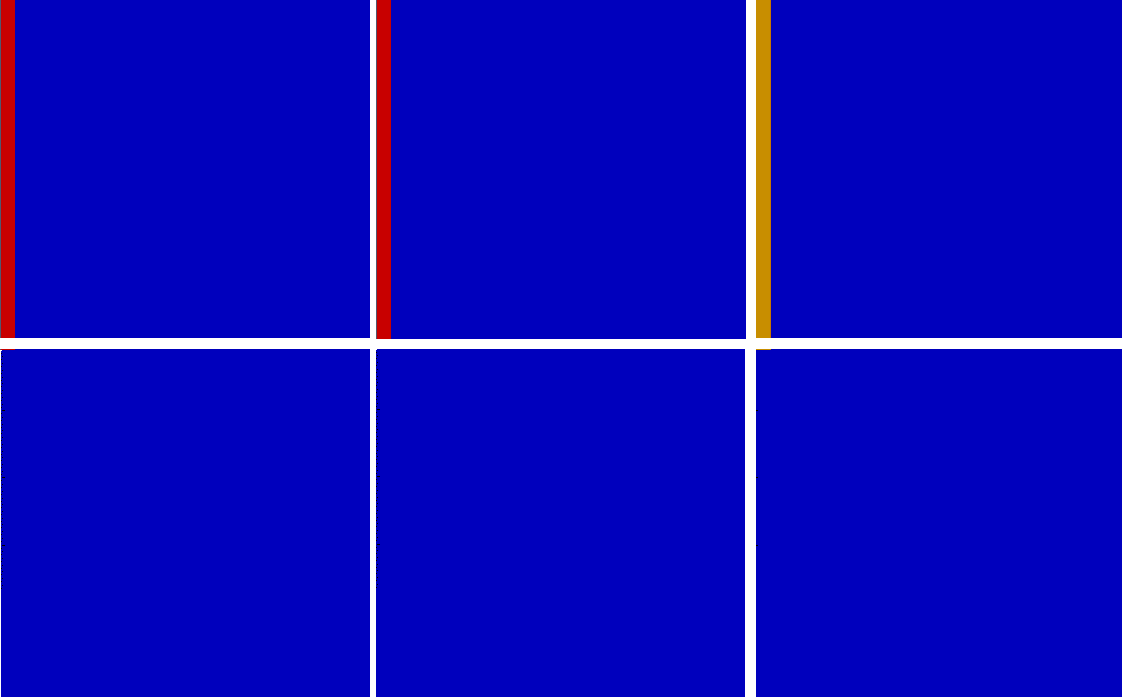
\includegraphics[height = 6 cm]{fig/Numerical_Experiments/ex3/results}
\caption{evolution of the potential over the tissue for the exact (up) and the homogenized (down) problem. From left to right, we have $t = 3~[ms]$, $t = 7~[ms]$ and $t = 15~[ms]$.} \label{fig:results_exp3}
\end{figure}

Note that homogenized solution reproduces the potential vertical blocking, which is natural considering the construction of the effective tensor. In summary, regards to the scale of study the result is satisfactory.

\subsection{Experiment \# 4: Tissue with Randomly Generated Fibrosis}

The collagen laminations are usually randomly distributed. In this example we try to emulate that by setting $\theta_c  \sim \mathcal{N}(\mu_c, \sigma_c)$ and $\theta_f \sim \mathcal{N}(\mu_f, \sigma_f)$, where $\sigma_c$ and $\mu_c$ are the mean and the standard deviation of a normal distribution. In particular, we will use the paramters of the table \ref{tab:ex4_parametros_random}:

\begin{figure}[!htbp]
	\centering
	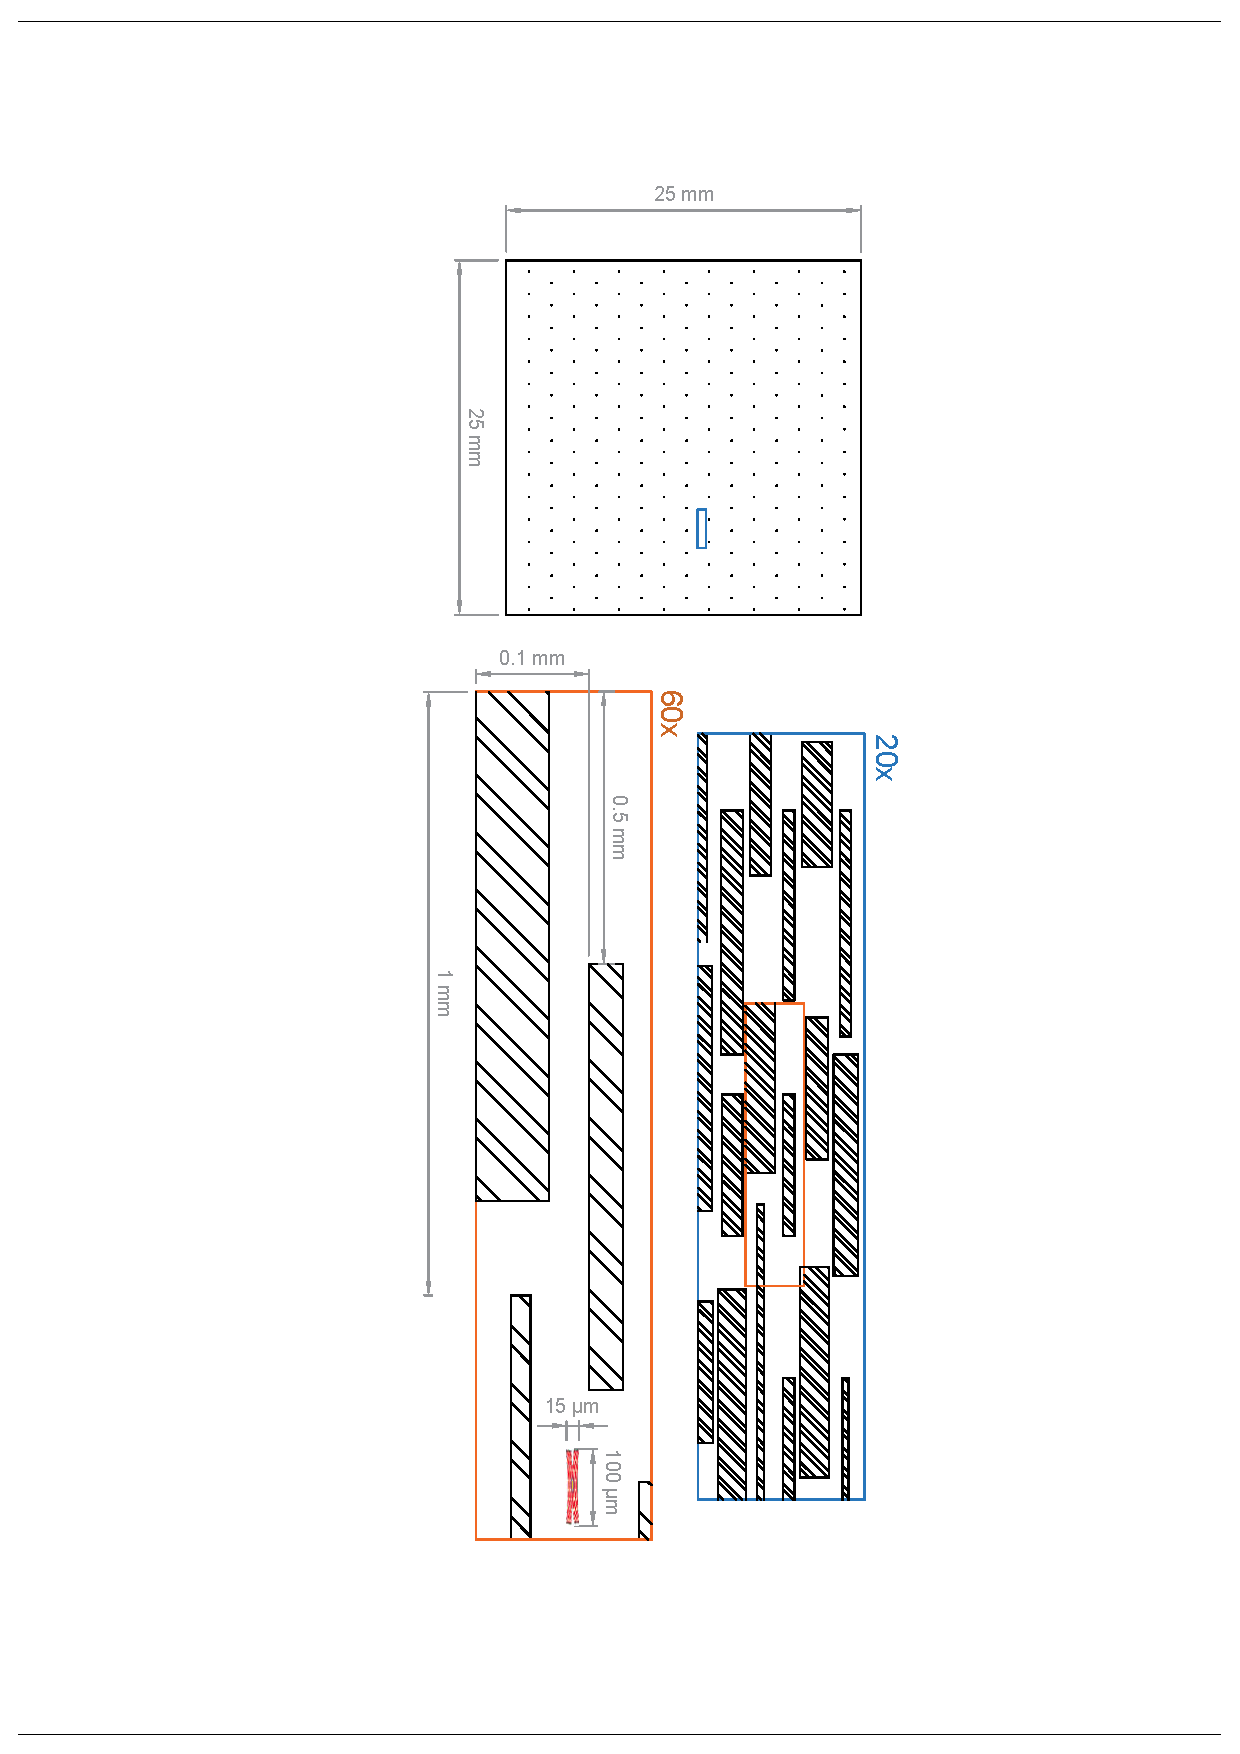
\includegraphics[trim={7cm 3.5cm 5.5cm 3cm}, clip, width = 6cm, angle = 90]{fig/Numerical_Experiments/ex4/geometry}
	\caption{Geometry for example \# 4.} \label{fig:ex3_random}
\end{figure}

Note that the $\mathbb{E}(\theta_c)$ and $\mathbb{E}(\theta_f)$ represents a tissue with moderated level of fibrosis. In the figure \ref{fig:ex3_random} the geometry generated with the parameters of table \ref{tab:ex4_parametros_random} can be observed.

If the random values are not within a physiological range are then recalculated. For $\theta_c$ we admit values from 0.15 (healthy tissue) to 0.45 (highly fibrotic tissue), and for $\theta_f$ we admit values from 0.35 to 0.9. The choose of $\theta_f$ is done in order to get a tissue that emulates diffuse fibrosis, because values over 0.9 tends to generate collagen block-walls, i.e., stringy fibrosis. In addition, this example consider a stimulus with Gaussian distribution shape, with its maximum value located in the left-down corner. This allow us to see how the tissue anisotropy affects the wave propagation process, and how the surrogate model deals with it.

\begin{table}[!htbp]
	\centering
	\caption{Parameters used to generate random fibrotic tissue mesh.}
	\label{tab:ex4_parametros_random}
	\begin{tabular}{@{}cc@{}}
		\toprule
		Parameter  & Value \\ \midrule
		$\mu_c$    & 0.3   \\
		$\mu_f$    & 0.5   \\
		$\sigma_c$ & 0.2   \\
		$\sigma_f$ & 0.3   \\ \bottomrule
	\end{tabular}
\end{table}

\subsubsection{Results Using FHN Reaction Model}


The results and error evolution are shown in the figure \ref{fig:ex4FHN} and \ref{fig:ex4MIN_error_L2}, respectively. 

\begin{figure}[!htbp]
	\centering
	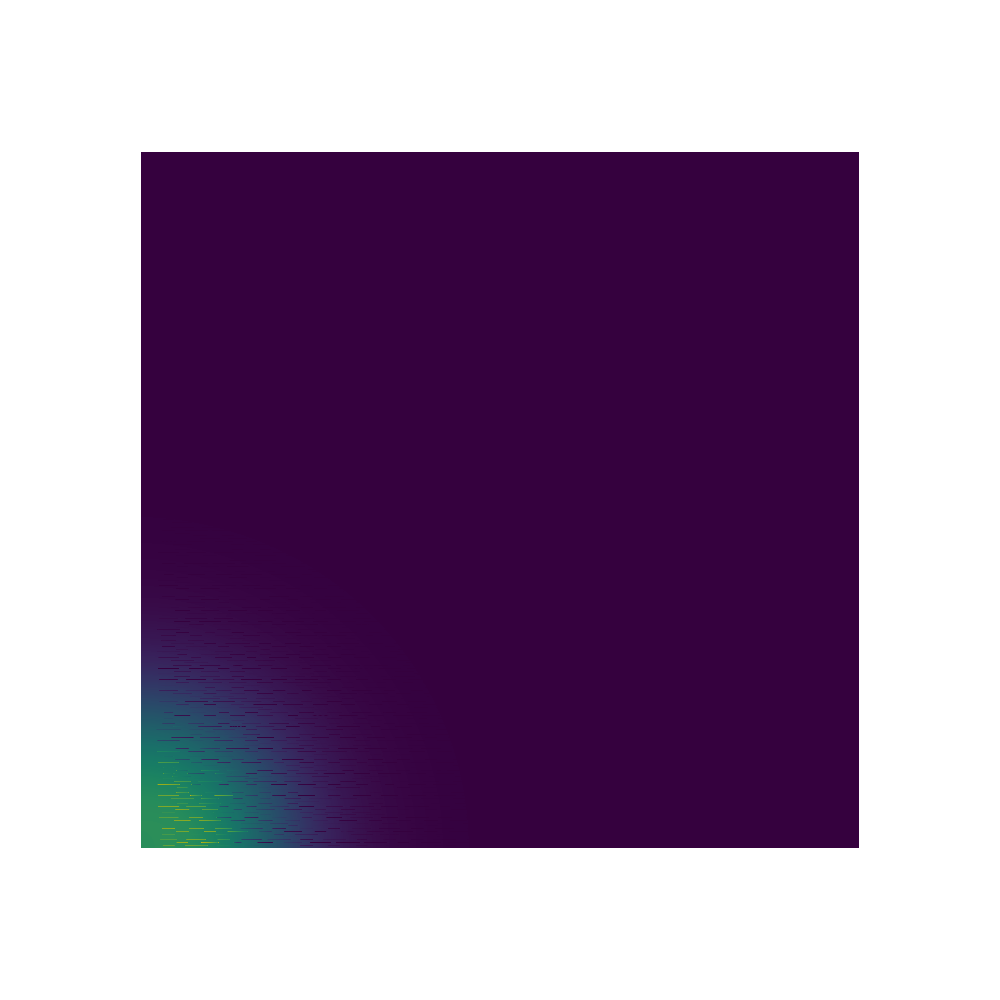
\includegraphics[height = 3 cm, trim = {6cm 6cm 6cm 6cm}, clip]{fig/Numerical_Experiments/ex4/FHN/100}
	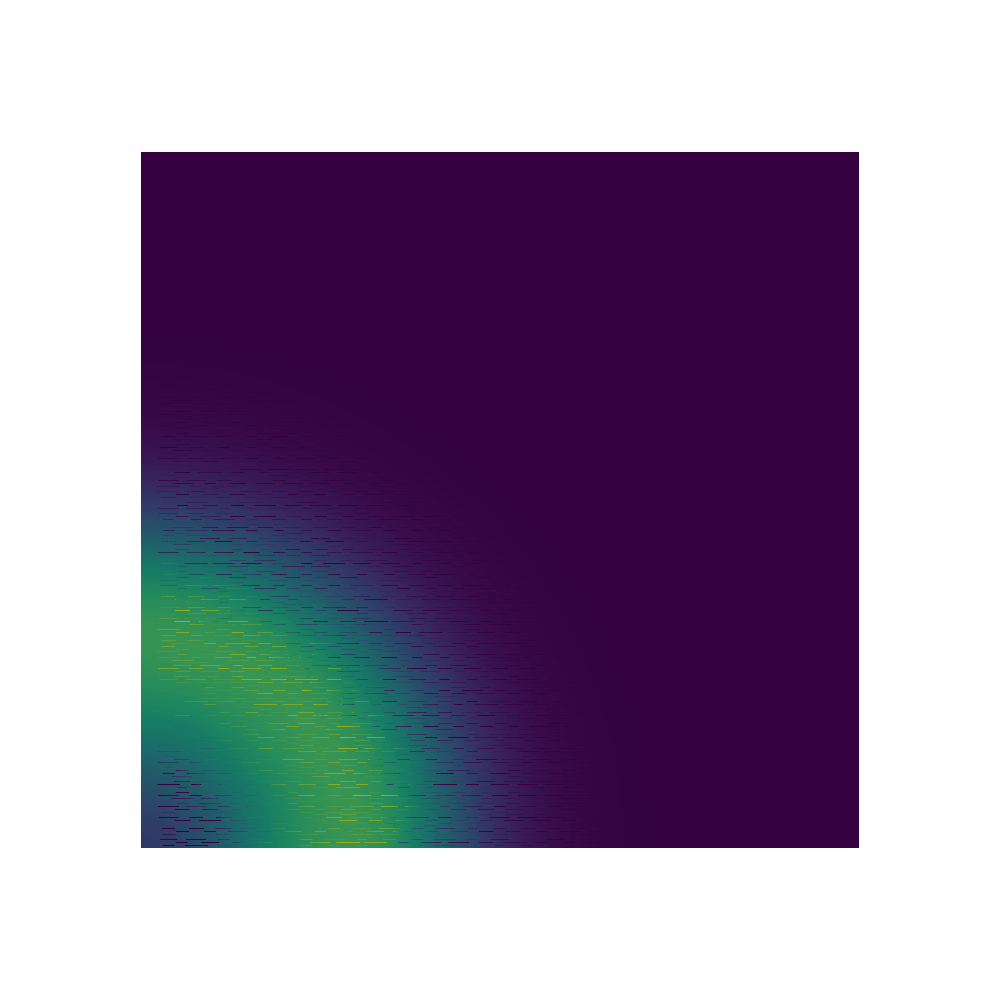
\includegraphics[height = 3 cm, trim = {6cm 6cm 6cm 6cm}, clip]{fig/Numerical_Experiments/ex4/FHN/300}
	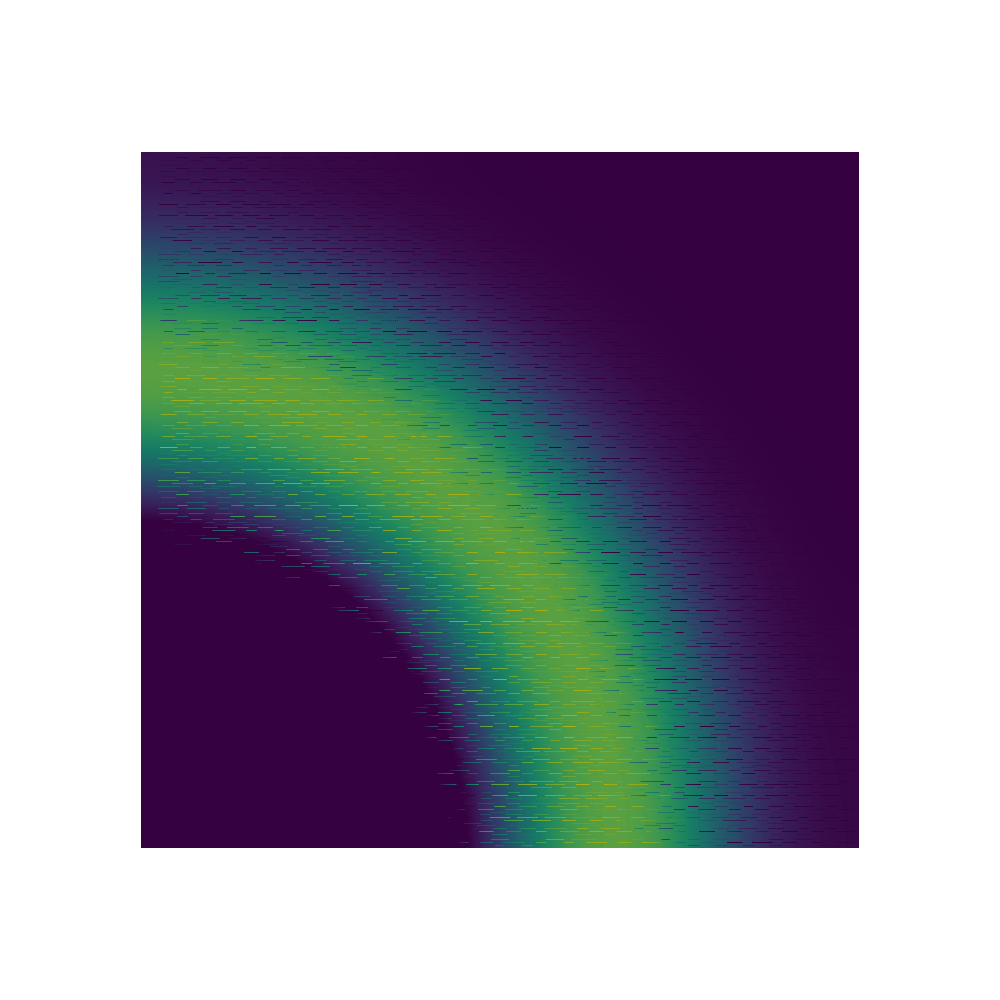
\includegraphics[height = 3 cm, trim = {6cm 6cm 6cm 6cm}, clip]{fig/Numerical_Experiments/ex4/FHN/500}
	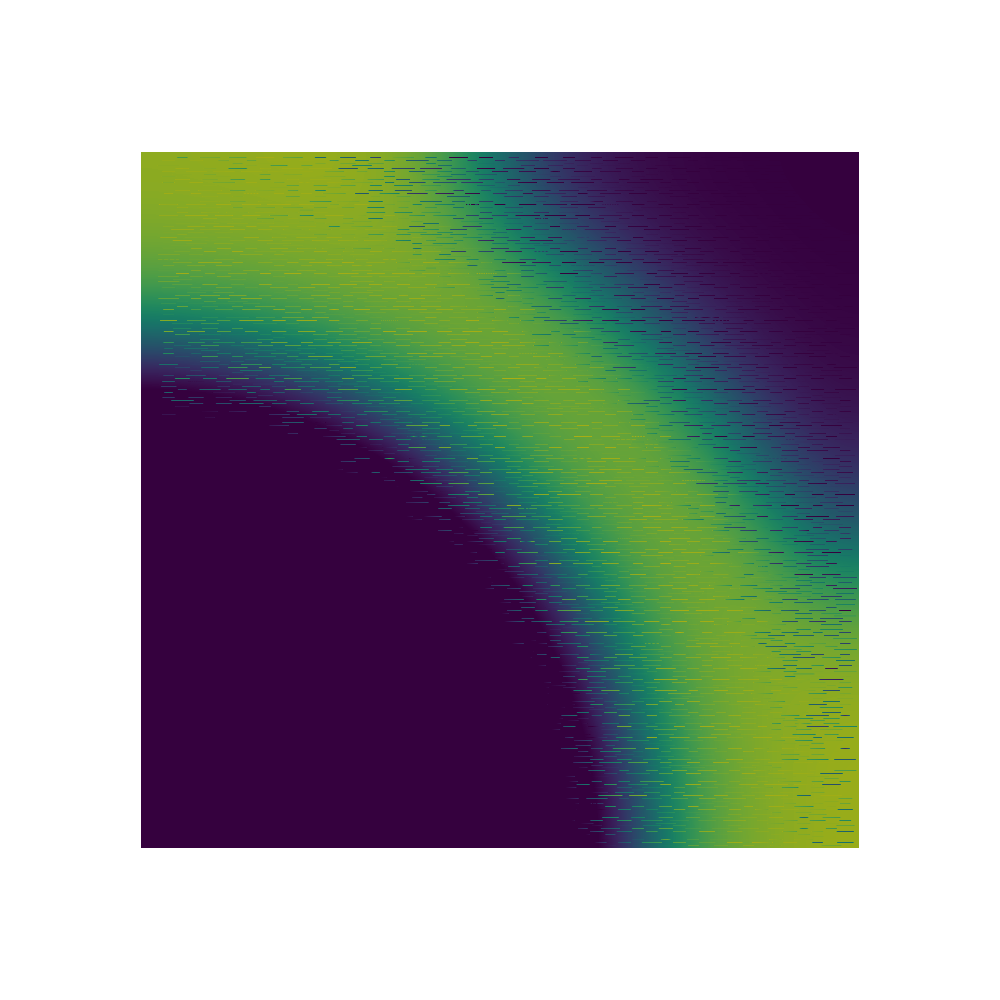
\includegraphics[height = 3 cm, trim = {6cm 6cm 6cm 6cm}, clip]{fig/Numerical_Experiments/ex4/FHN/600} \\[0.1 cm]
	
\includegraphics[height = 3 cm, trim = {6cm 6cm 6cm 6cm}, clip]{fig/Numerical_Experiments/ex4/FHN/100h}
	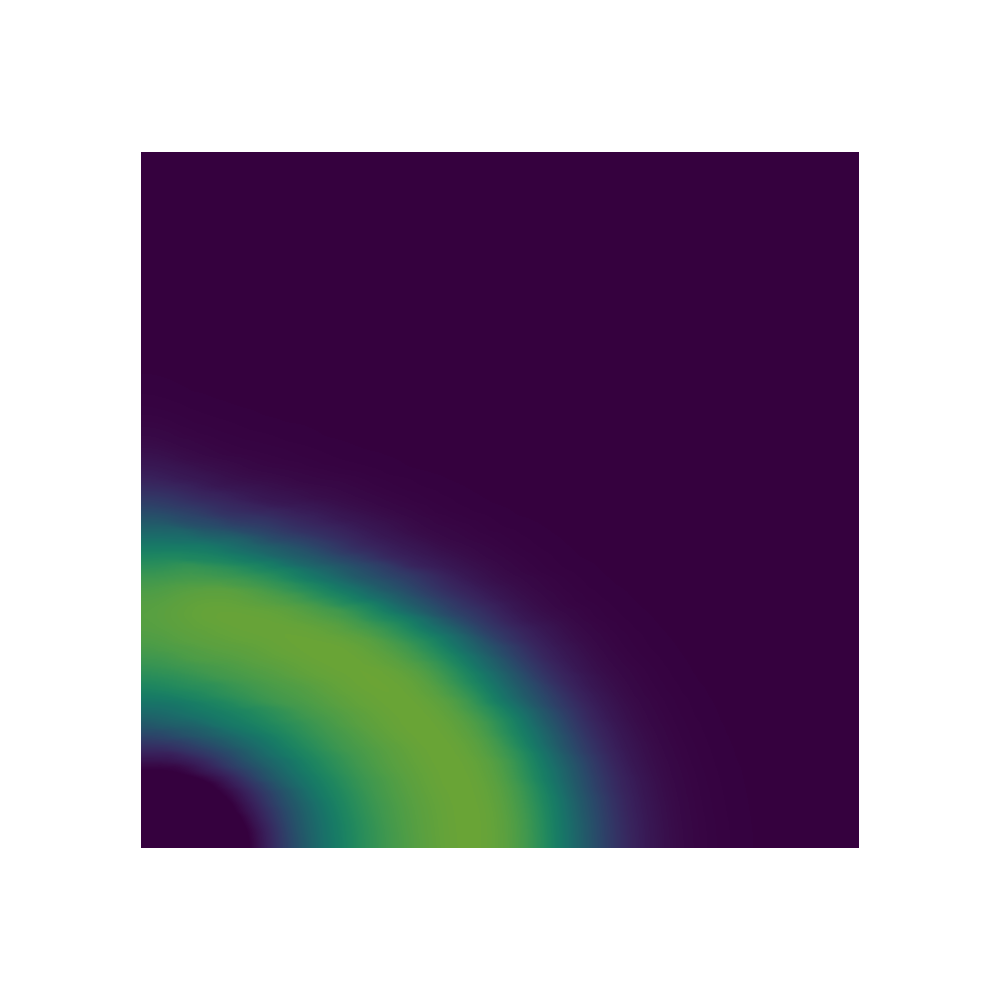
\includegraphics[height = 3 cm, trim = {6cm 6cm 6cm 6cm}, clip]{fig/Numerical_Experiments/ex4/FHN/300h}
	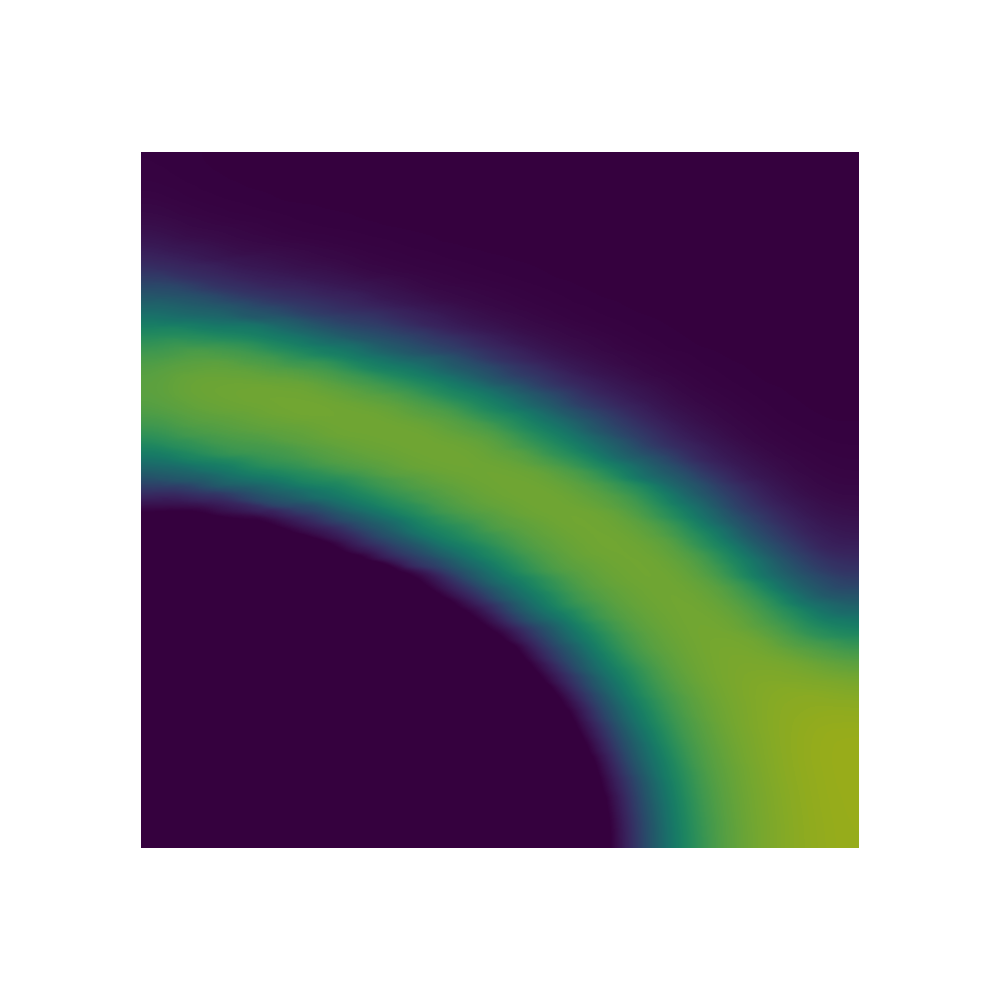
\includegraphics[height = 3 cm, trim = {6cm 6cm 6cm 6cm}, clip]{fig/Numerical_Experiments/ex4/FHN/500h}
	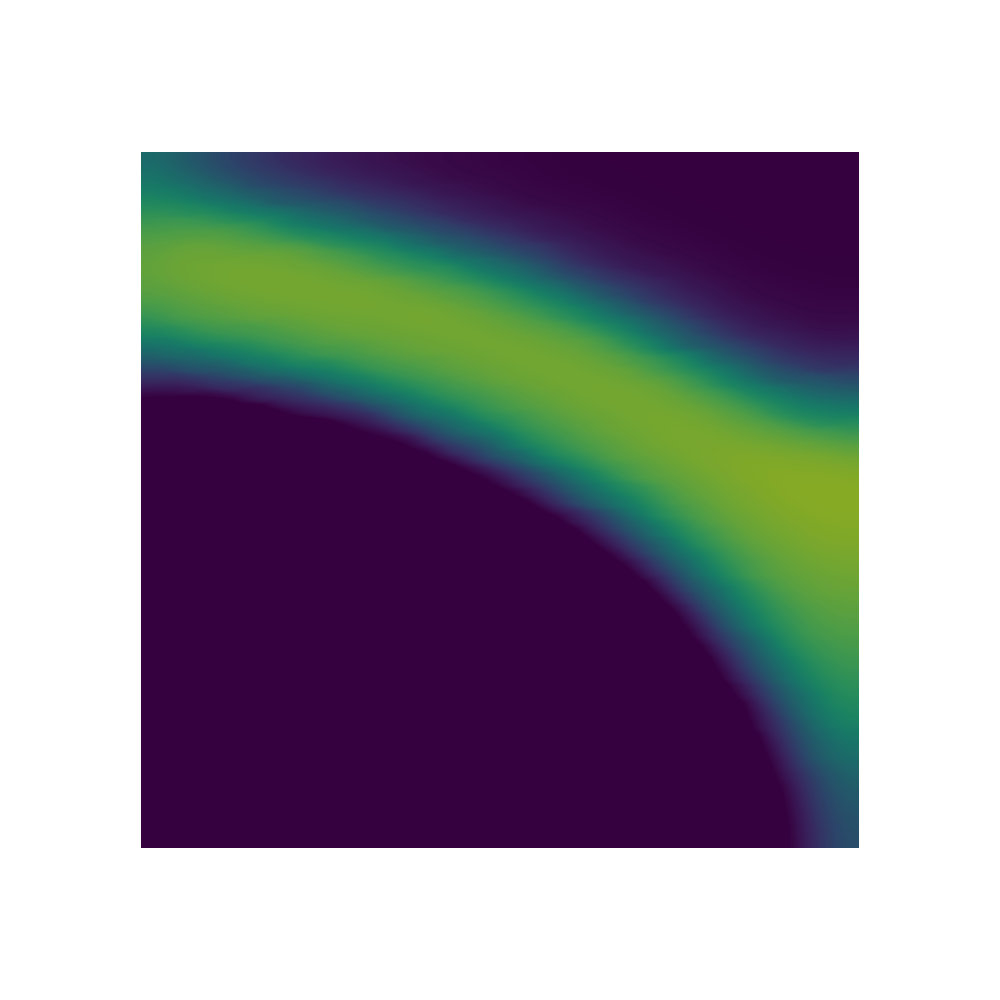
\includegraphics[height = 3 cm, trim = {6cm 6cm 6cm 6cm}, clip]{fig/Numerical_Experiments/ex4/FHN/600h}  \\[0.3 cm]
	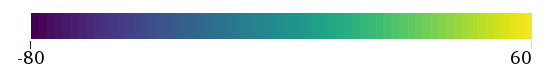
\includegraphics[height = 0.9 cm]{fig/Numerical_Experiments/colourbar_FHN}	
	\caption{Temporal evolution of the exact (up) and the homogenized (down) solution. From left to right we have $t = 100 ms$, $t = 300 ms$,  $t = 500 ms$ and $t = 600 ms$} \label{fig:ex4FHN}
\end{figure}



\begin{figure}[!htbp]
	\centering
	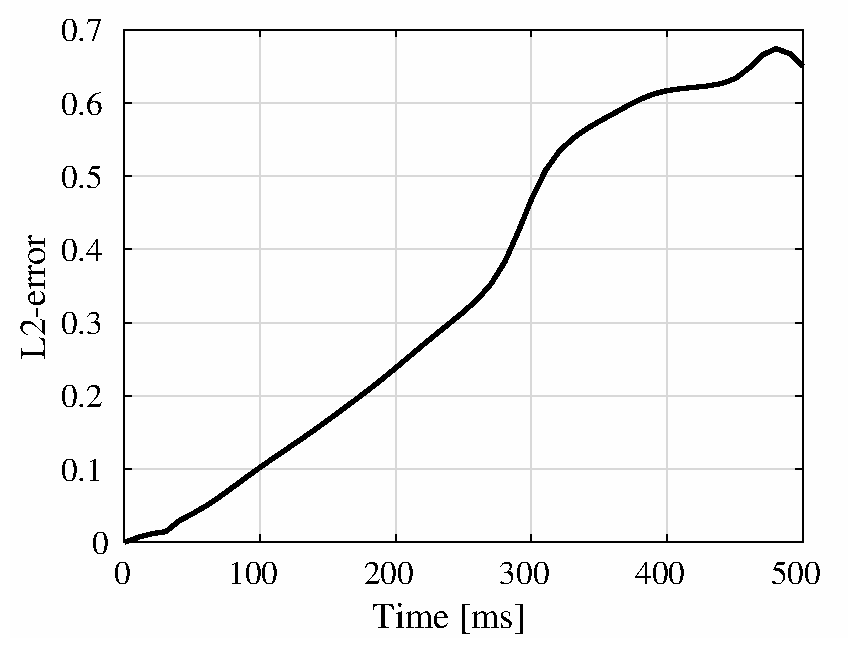
\includegraphics[height = 5 cm]{fig/Numerical_Experiments/ex4/FHN/error_L2.eps}
	\caption{Temporal evolution of the error.}
	\label{fig:ex4MIN_error_L2}
\end{figure}


\subsubsection{Results Using Minimal Reaction Model}

The results for an Atrial tissue are shown in the figure \ref{fig:ex4Min} and the error is in figure \ref{fig:ex4_error_L2}. We can see an increase in the L2-error respect to the non-random case, which is a consequence of the experiment configuration. Notice that the wave propagation in the surrogate model fits better with the exact solution across the fiber direction than in the cross-fiber direction. This difference can be explained by considering the tissue anisotropy and the material proportions. In the fiber direction the collagen proportion at the meso-scale is smaller than in the vertical direction, therefore a better fit with the surrogate model in the fiber direction is expected.


\begin{figure}[!htbp]
	\centering
	
\includegraphics[height = 3 cm, trim = {6cm 6cm 6cm 6cm}, clip]{fig/Numerical_Experiments/ex4/MINIMAL/3}
	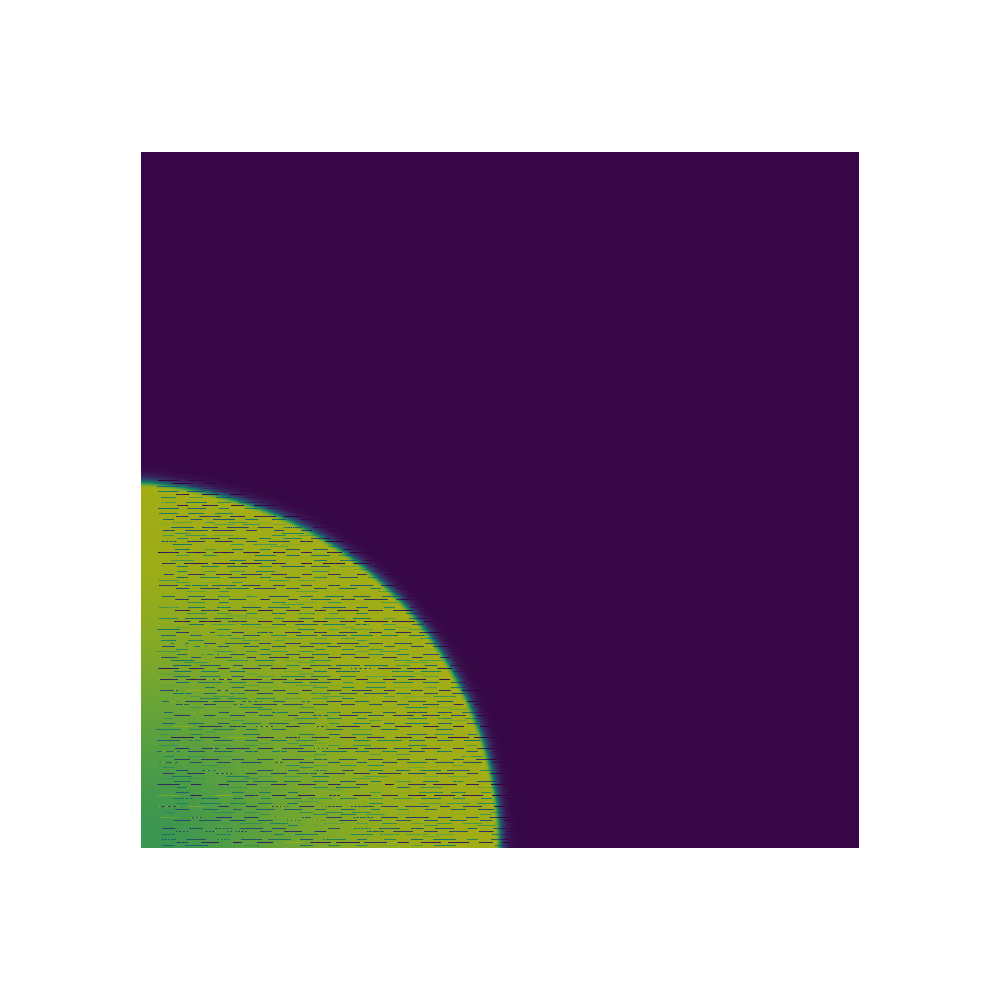
\includegraphics[height = 3 cm, trim = {6cm 6cm 6cm 6cm}, clip]{fig/Numerical_Experiments/ex4/MINIMAL/10}
	\includegraphics[height = 3 cm, trim = {6cm 6cm 6cm 6cm}, clip]{fig/Numerical_Experiments/ex4/MINIMAL/20}
	\includegraphics[height = 3 cm, trim = {6cm 6cm 6cm 6cm}, clip]{fig/Numerical_Experiments/ex4/MINIMAL/35} \\[0.1 cm]
	\includegraphics[height = 3 cm, trim = {6cm 6cm 6cm 6cm}, clip]{fig/Numerical_Experiments/ex4/MINIMAL/3h}
	\includegraphics[height = 3 cm, trim = {6cm 6cm 6cm 6cm}, clip]{fig/Numerical_Experiments/ex4/MINIMAL/10h}
	\includegraphics[height = 3 cm, trim = {6cm 6cm 6cm 6cm}, clip]{fig/Numerical_Experiments/ex4/MINIMAL/20h}
	\includegraphics[height = 3 cm, trim = {6cm 6cm 6cm 6cm}, clip]{fig/Numerical_Experiments/ex4/MINIMAL/35h}  \\[0.3 cm]
	\includegraphics[height = 0.9 cm]{fig/Numerical_Experiments/colourbar_MINIMAL}	
	\caption{Temporal evolution of the exact (up) and the homogenized (down) solution. From left to right we have $t = 3 ms$, $t = 10 ms$,  $t = 20 ms$ and $t = 35 ms$} \label{fig:ex4Min}
\end{figure}


\begin{figure}[!htbp]
\centering
\includegraphics[height = 5 cm]{fig/Numerical_Experiments/ex4/MINIMAL/error_L2.eps}
\caption{Temporal evolution of the error.}
\label{fig:ex4_error_L2}
\end{figure}



\section{Conclusion and Perspectives}

We successfully obtained a model for the electric potential propagation in cardiac human tissue based on a classical reaction-diffusion approach using both FitzHugh-Nagumo and Minimal reaction terms. For future research, in order to get realistic enough simulations for the membrane cell activity regards to AP duration, AP shape and refractory time properties  we will consider the Minimal model only. Also, we can couple the Monodomain equations with a mechanical model for the cardiac tissue, since myocites has very elastic properties that affects the potential propagation.

The homogenization theory gives a very useful and effective tool to deal with fibered materials. By using some results of this theory, we obtained a surrogate model that severely improve the computational performance of the simulations, preserving the meso-scale properties in a mesh that only consider the macro-scopic scale. This surrogate model works fine for different configurations of fibrosis types, such as diffuse fibrosis and stringy fibrosis.

For future work, it will be necessary to apply the homogenization results in a three dimensional realistic geometry, considering the spatial variation of the lamination direction. Also, in order to evaluate the behavior of surrogate model in arrhythmia situations as a consequence of fibrosis, we have to study the spiral wave generation and break-up in cardiac tissue and see how the homogenized problem reproduces it.

Once we have all the above, one can go further and develop the inverse version of the electro-physiology problem, then use real electric potential measures to asses the fibrosis architecture and level of real patients, achieving finally a non-invasive way to diagnose pathological fibrosis.

As a final remark, it has to be noted that on this text we developed a tool for any kind of fibered material. Therefore, we can go beyond our bio-medical example and look for new applications of the surrogate model, wherever those materials arises.